\chapter{Results}\label{chap:results}
Based on the metrics discussed in \hyperref[sec:evaluation_metrics]{Section~\ref*{sec:evaluation_metrics}}, this chapter highlights the results of our evaluation.
It is divided along the datasets we used for evaluation, that is, \hyperref[sec:result_cc_ontology]{Section~\ref*{sec:result_cc_ontology}} covers the \emph{climate~change} domain, \hyperref[sec:result_f_ontology]{Section~\ref*{sec:result_f_ontology}} is dedicated to \emph{finance} and \emph{tennis} is handled in \hyperref[sec:result_t_ontology]{Section~\ref*{sec:result_t_ontology}}. Finally, an overall \emph{comparison} of all evaluation domains is done in \hyperref[sec:result_comparison]{Section~\ref*{sec:result_comparison}}.


%%%%%%%%%%%%%%%%%%%%%%%%%%%%%%%%%%%%%%%%%%%%%%%%%%%%%%%%%%%%%%%%%%%%%%%%%%%%%%%%%%%%%%%%%%%%%%%%%%%%%%%%%%%%%%%%%%%%%%%%%%%%%%%%%%%%%%%%%%%%%%%%%%%%

% SECTION: CLIMATE CHANGE ONTOLOGY %
\section{Climate Change Ontology}\label{sec:result_cc_ontology}
In this section, results from the crowd-sourced ontology validation in the field of climate change are presented. A detailed discussion of the ontology used as a baseline for all calculations was done previously in \hyperref[sec:evaluation_datasets]{Section~\ref*{sec:evaluation_datasets}}. 

The results of the benchmark are presented in~\hyperref[table:bench_p_r_f_climate_change]{Table~\ref*{table:bench_p_r_f_climate_change}}. For comparison, we also performed ontology validation without any of the discussed Context enrichment methods~\emph{(None)}. Given the relatively small number of concepts, all Context enrichment methods performed better than having no Context at all. Surprisingly, in terms of Recall the contrary holds. Indeed, crowd workers tend to negatively answer questions in case of uncertainty or when no additional information other than the concept name is present. 
\begingroup
\renewcommand{\arraystretch}{1.5}
\begin{table}
	\begin{tabularx}{\textwidth}{l c*{3}{Y}}
		\toprule
		Method & Precision & Recall & F-Measure \\
		\midrule
		 Neighbouring Nodes & 0.758 & 0.805 & 0.781 \\
		 Embedded Context & 0.732 & 0.831 & 0.778 \\
		 External Source & 0.724 & 0.821 & 0.769 \\
		 None & 0.549 & 0.837 & 0.663 \\
		\bottomrule
	\end{tabularx}
	\caption{Aggregated results on the Climate Change Ontology~(ranked by F-Measure)}
	\label{table:bench_p_r_f_climate_change}
\end{table}
\endgroup

We also measured the agreement ratio~(Inter-rater Agreement) in this dataset. \hyperref[fig:hist_agreement_climate_change_all]{Figure~\ref*{fig:hist_agreement_climate_change_all}} shows the distribution of the agreement ratio among all validated concepts. We required 5 judgements for every concept, yielding $5/0$, $4/1$ or $3/2$ levels of agreement, which is equivalent to
\emph{full agreement}~($1.0$), \emph{partial agreement}~($0.8$) and \emph{little agreement}~($0.6$) respectively. 
\begin{sidewaysfigure}
  	 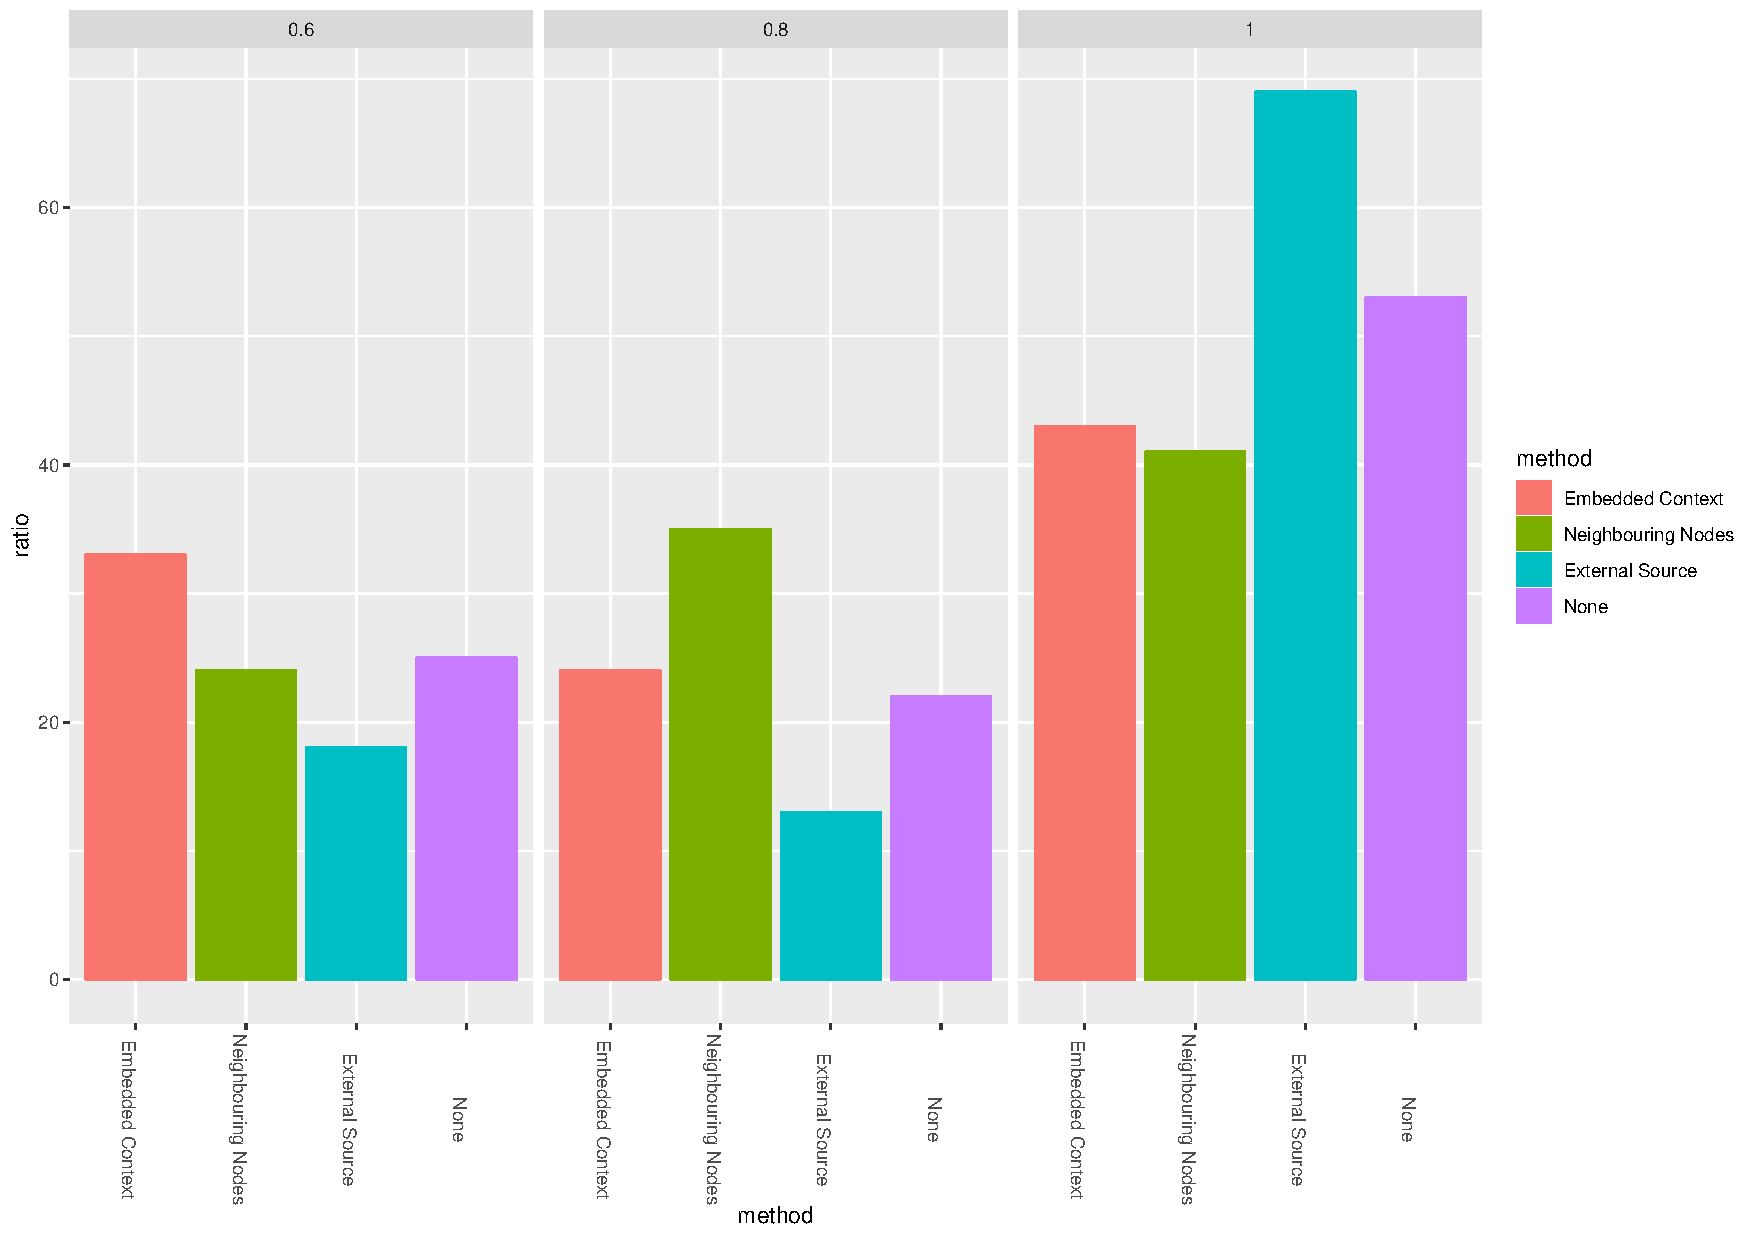
\includegraphics[width=\textwidth]{plots/climate_change/hist_agreement}
  	 \caption{Histogram plots of the Inter-rater Agreement}\label{fig:hist_agreement_climate_change_all}
\end{sidewaysfigure}

The highest agreement exhibits \emph{External~Source}, followed by \emph{None}. This is somewhat interesting as these are the methods with the lowest performance with regard to F-Measure. In fact, the agreement ratio just describes to what extent the responses coincide. From the observations in this dataset, it is hard, if not impossible, to draw conclusions solely based on agreement. In fact, when looking closely at the judgements with the highest agreement~ratio among incorrect answers, $16$ of $17$ judgements for External~Source and $3$ of $6$ judgements for Neighbouring~Nodes had Context added. Apparently, crowd workers agreed here on incorrect values even though that concept descriptions were available. 

\begin{figure}
    \centering
    \begin{subfigure}[b]{0.4\textwidth}
        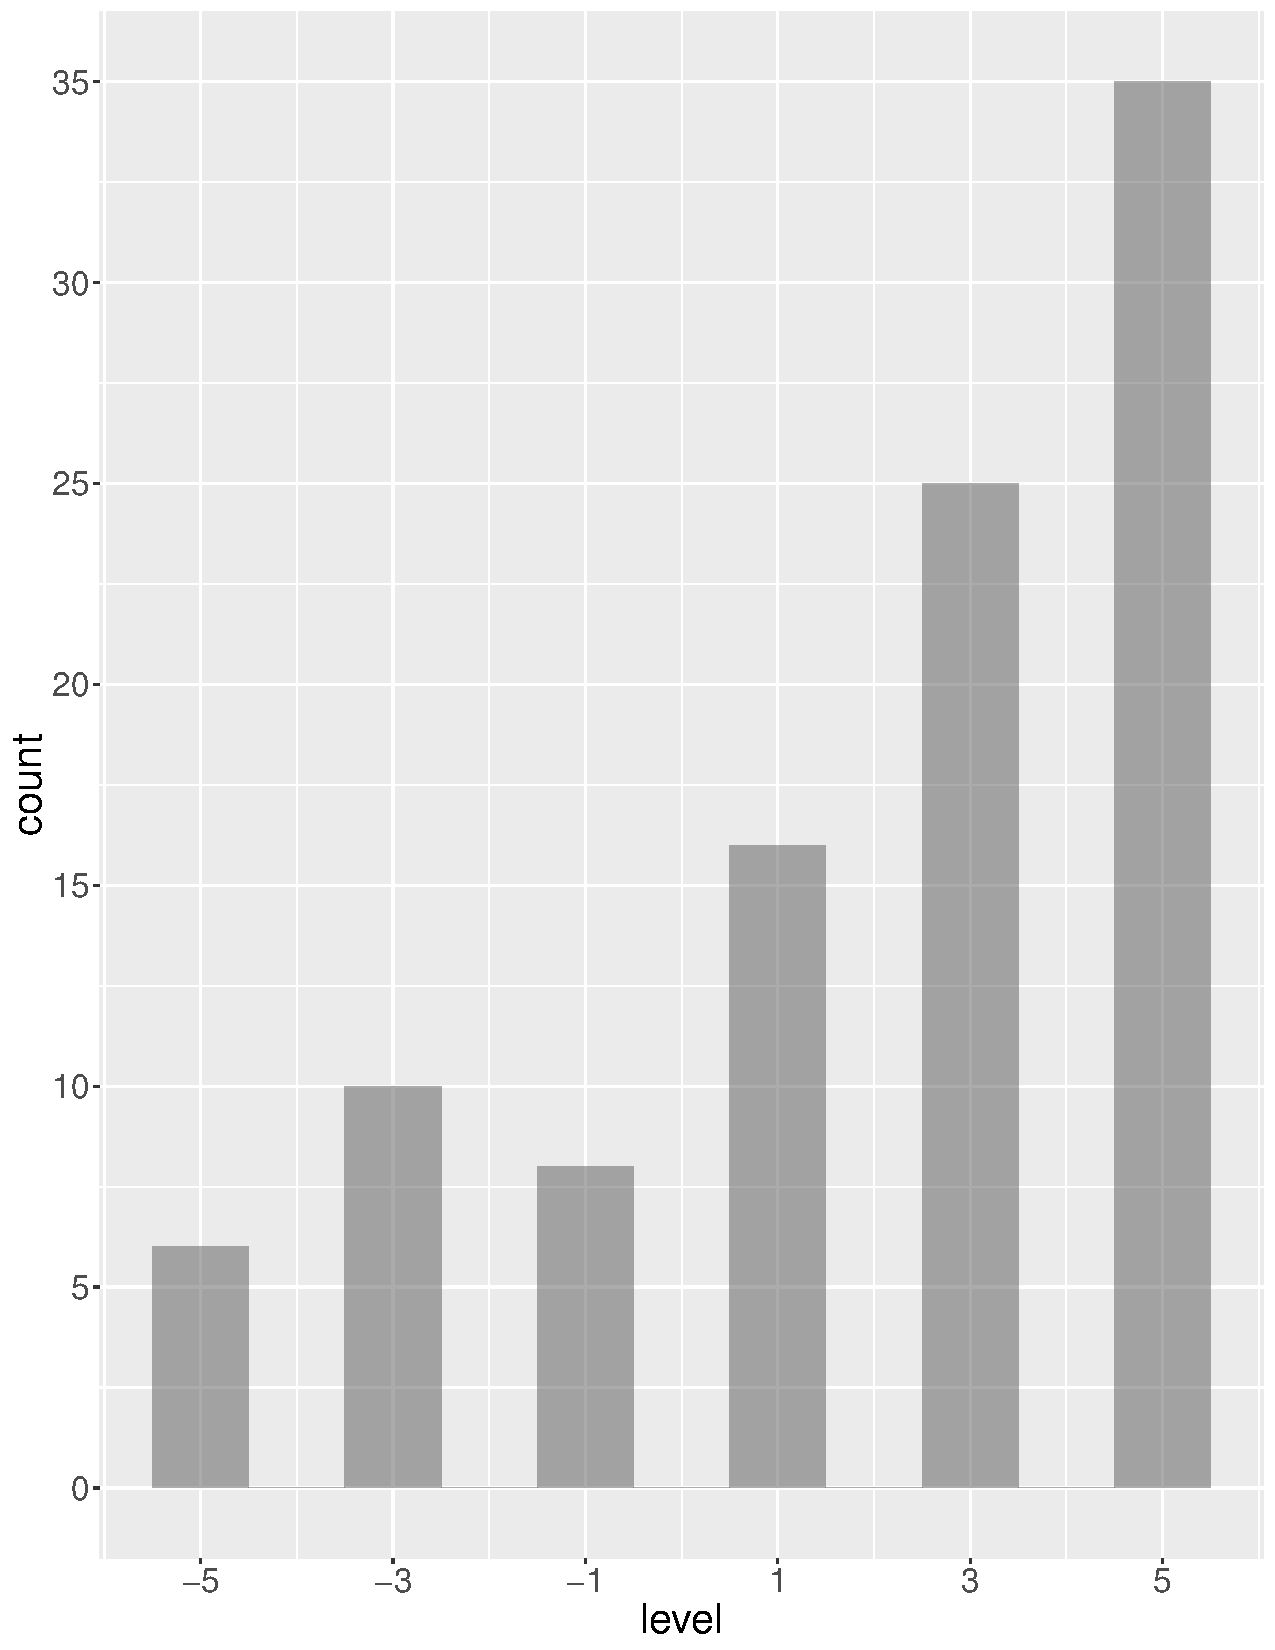
\includegraphics[width=\textwidth]{plots/climate_change/hist_level_nn}
        \caption{Neighbouring Nodes}
        \label{fig:hist_level_climate_change_nn}
    \end{subfigure}
    ~
    \begin{subfigure}[b]{0.4\textwidth}
        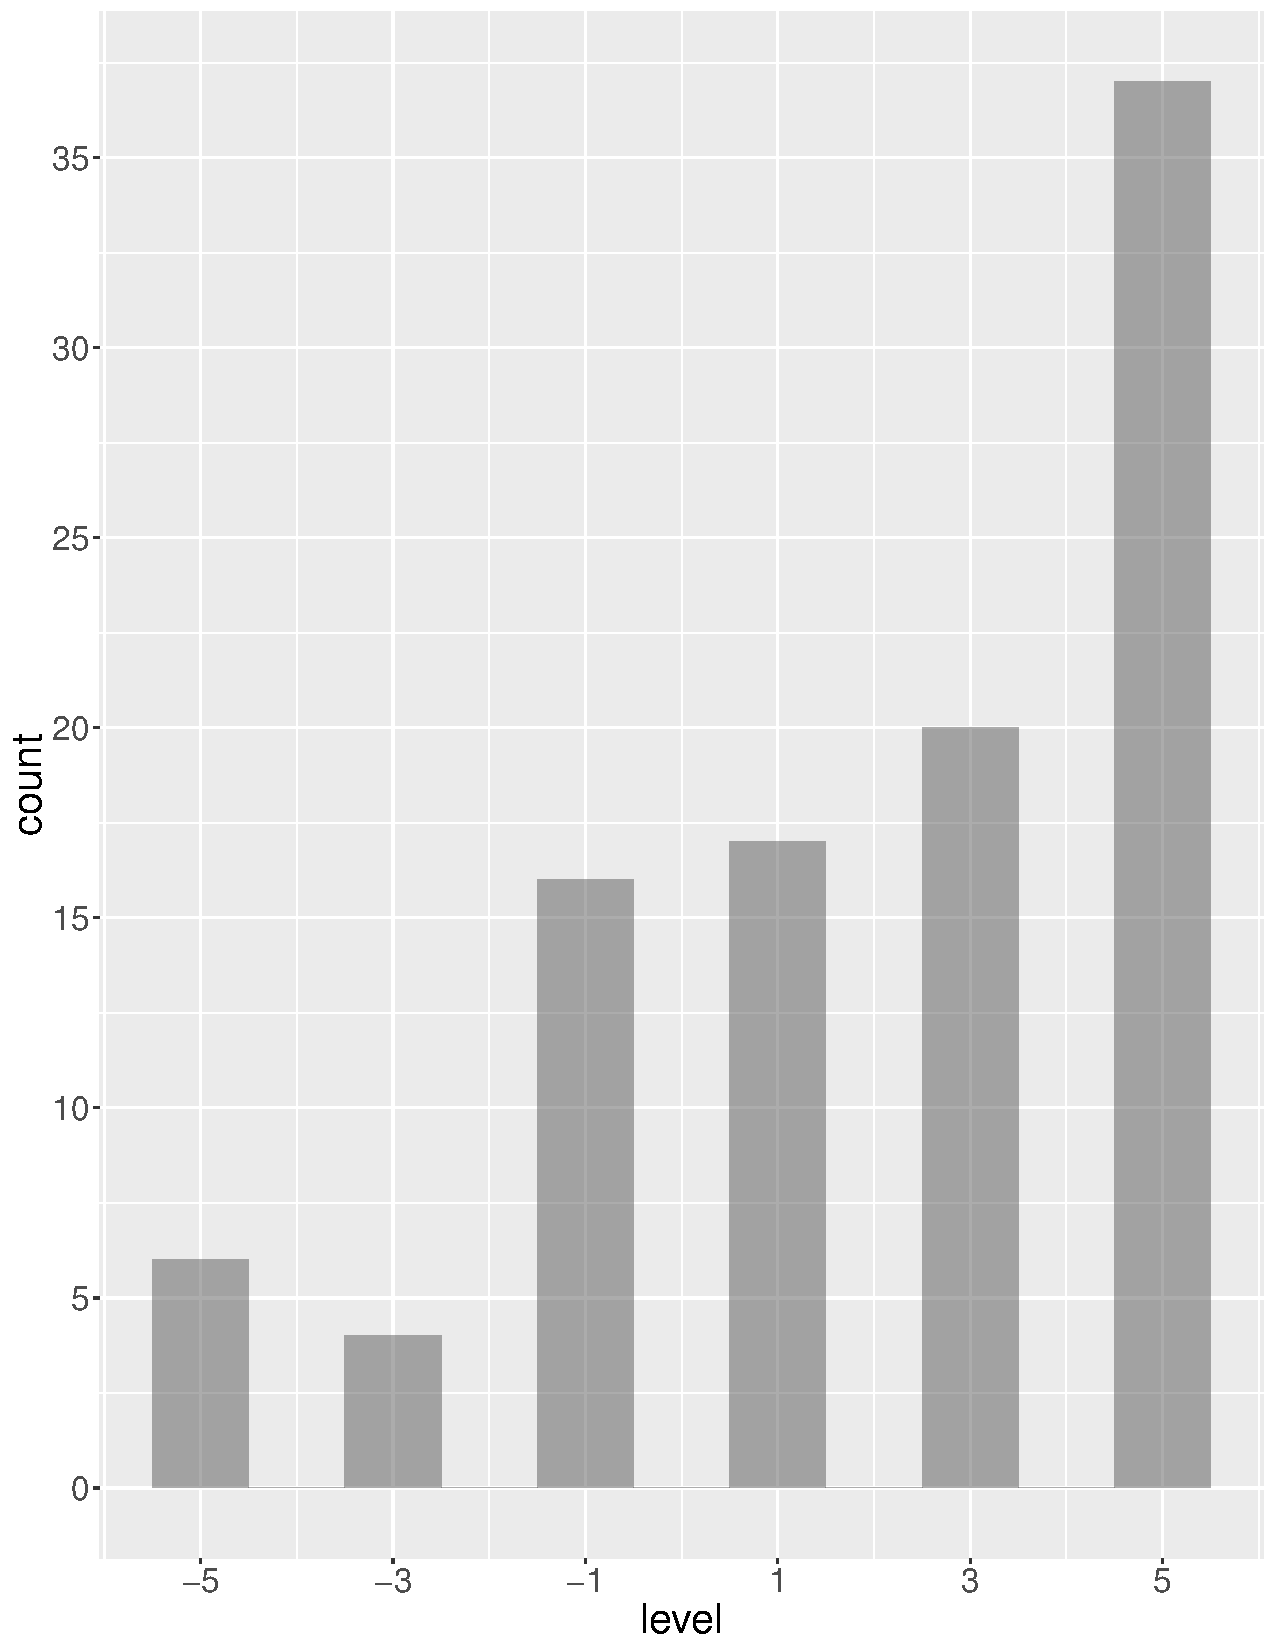
\includegraphics[width=\textwidth]{plots/climate_change/hist_level_ec}
        \caption{Embedded Context}
        \label{fig:hist_level_climate_change_ec}
    \end{subfigure}
    ~
    \begin{subfigure}[b]{0.4\textwidth}
        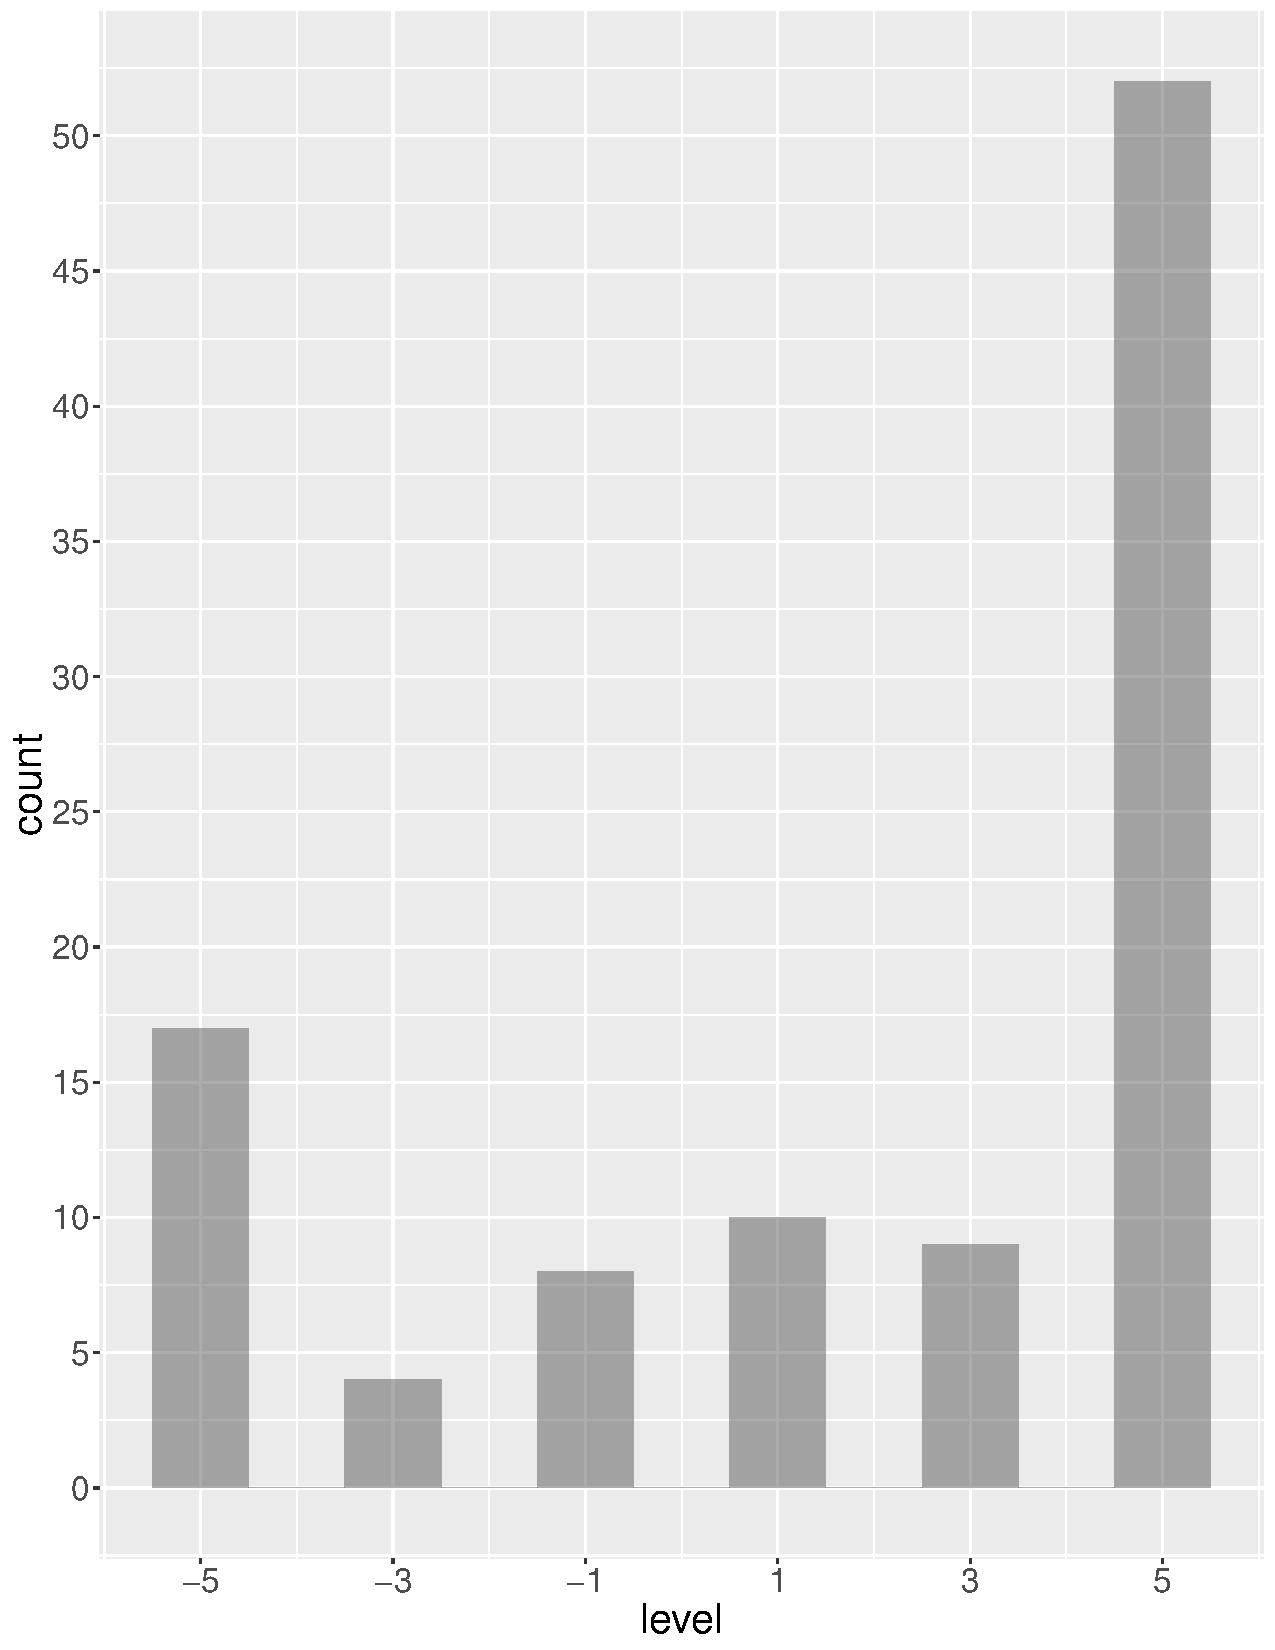
\includegraphics[width=\textwidth]{plots/climate_change/hist_level_es}
        \caption{External Source}
        \label{fig:hist_level_climate_change_es}
    \end{subfigure}
    ~
    \begin{subfigure}[b]{0.4\textwidth}
        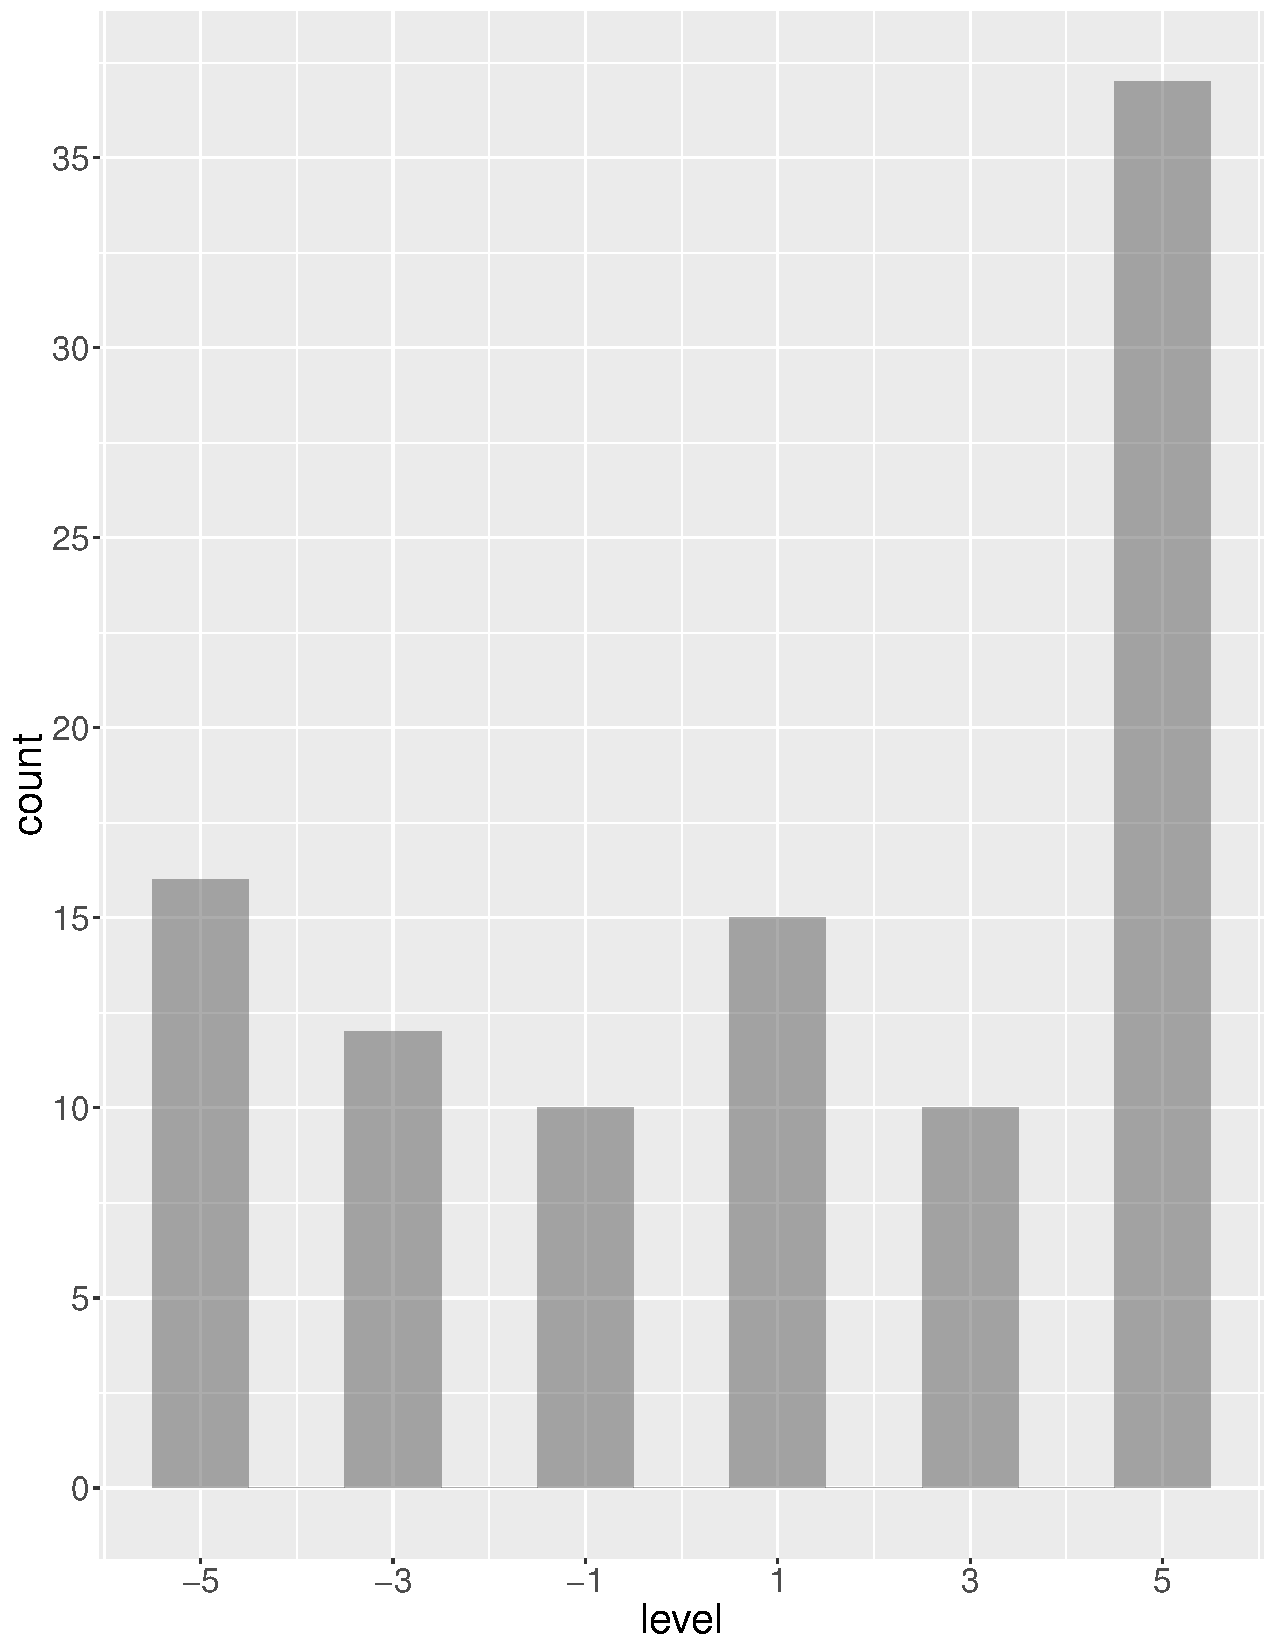
\includegraphics[width=\textwidth]{plots/climate_change/hist_level_none}
        \caption{None}
        \label{fig:hist_level_climate_change_none}
    \end{subfigure}
    \caption{Histogram plots of the correct/incorrect judgements}\label{fig:hist_level_climate_change_all}
\end{figure}

To manifest our observations from above, bar plots~(illustrated in \hyperref[fig:hist_level_climate_change_all]{Figure~\ref*{fig:hist_level_climate_change_all}}) were created. It combines the agreement ratio with the amount of correct/incorrect judgements. Whereas a negative score indicates that more contributors agreed on incorrect answers or declined relevant concepts, a positive score shows that the majority of crowd worker's responses were correct. Indeed, when comparing the performance on level $-5$ \emph{External~Source} is on the same level as if Context was omitted. On the other hand, it shows the highest score of correct answers on level $5$.

Given the plots on the distribution of the correct/incorrect judgements from above, \hyperref[table:level_corr_incorr_climate_change]{Table~\ref*{table:level_corr_incorr_climate_change}} shows the summary statistics of agreement levels for each Context enrichment method. It confirms our observations made so far.
\begingroup
\renewcommand{\arraystretch}{1.5}
\begin{table}
	\begin{tabularx}{\textwidth}{l c*{4}{Y}}
		\toprule
		Method & mean & median & $1^{st}$ quartile & $3^{rd}$ quartile \\
		\midrule
		 Embedded Context & 2.04 & 3.00 & -1.00 & 5.00 \\
		 Neighbouring Nodes & 1.98 & 3.00 & 1.00 & 5.00 \\
		 External Source & 1.92 & 5.00 & -1.00 & 5.00 \\
		 None & 1.04 & 1.00 & -3.00 & 5.00 \\
		\bottomrule
	\end{tabularx}
	\caption{Summary statistics concerning agreement level on the Climate Change Ontology~(ranked by mean value)}
	\label{table:level_corr_incorr_climate_change}
\end{table}
\endgroup


% SECTION: FINANCE ONTOLOGY %
\section{Finance Ontology}\label{sec:result_f_ontology}
In this section, results from the crowd-sourced ontology validation in the domain of finance are presented. A detailed discussion of the ontology used as a baseline for all calculations was done previously in \hyperref[sec:evaluation_datasets]{Section~\ref*{sec:evaluation_datasets}}.

As with the other datasets the~\emph{Metadata based Approach} performed quite well. In fact, it outperformed all other approaches, both in terms of Precision and Recall, yielding the highest value of F-Measure. A detailed comparison of all methods for this dataset is given in~\hyperref[table:bench_p_r_f_finance]{Table~\ref*{table:bench_p_r_f_finance}}. On the other end of the table is ontology validation without any Context enrichment~(\emph{None}). This is in line with our initial hypothesis that motivated the use of concept descriptions. We also noticed the relatively high number of Recall for all approaches. The same observation was made for the other datasets as well. Indeed, crowd workers tend to decline concepts in case of uncertainty or lack of additional information.
\begingroup
\renewcommand{\arraystretch}{1.5}
\begin{table}
	\begin{tabularx}{\textwidth}{l c*{3}{Y}}
		\toprule
		Method & Precision & Recall & F-Measure \\
		\midrule
		 Metadata based Approach & 0.797 & 0.985 & 0.881 \\
		 Dictionary based Approach & 0.794 & 0.944 & 0.862 \\
		 Ontology based Approach & 0.756 & 0.949 & 0.842 \\
		 None & 0.734 & 0.963 & 0.833 \\
		\bottomrule
	\end{tabularx}
	\caption{Aggregated results on the Finance Ontology~(ranked by F-Measure)}
	\label{table:bench_p_r_f_finance}
\end{table}
\endgroup

Another metric we used to measure the performance of ontology validation was Inter-rater agreement. 
\hyperref[fig:hist_agreement_finance_all]{Figure~\ref*{fig:hist_agreement_finance_all}} depicts the distribution of the agreement ratio among all validated concepts. For comparability, all methods were merged into one chart and grouped by the level of agreement. Again, the~\emph{Metadata based Approach} performed best followed by the~\emph{Ontology~based~Approach} as indicated by the red bar. It shows both, a high level of full agreement~($1$) and low level of little agreement~($0.6$). 
\begin{sidewaysfigure}
  	 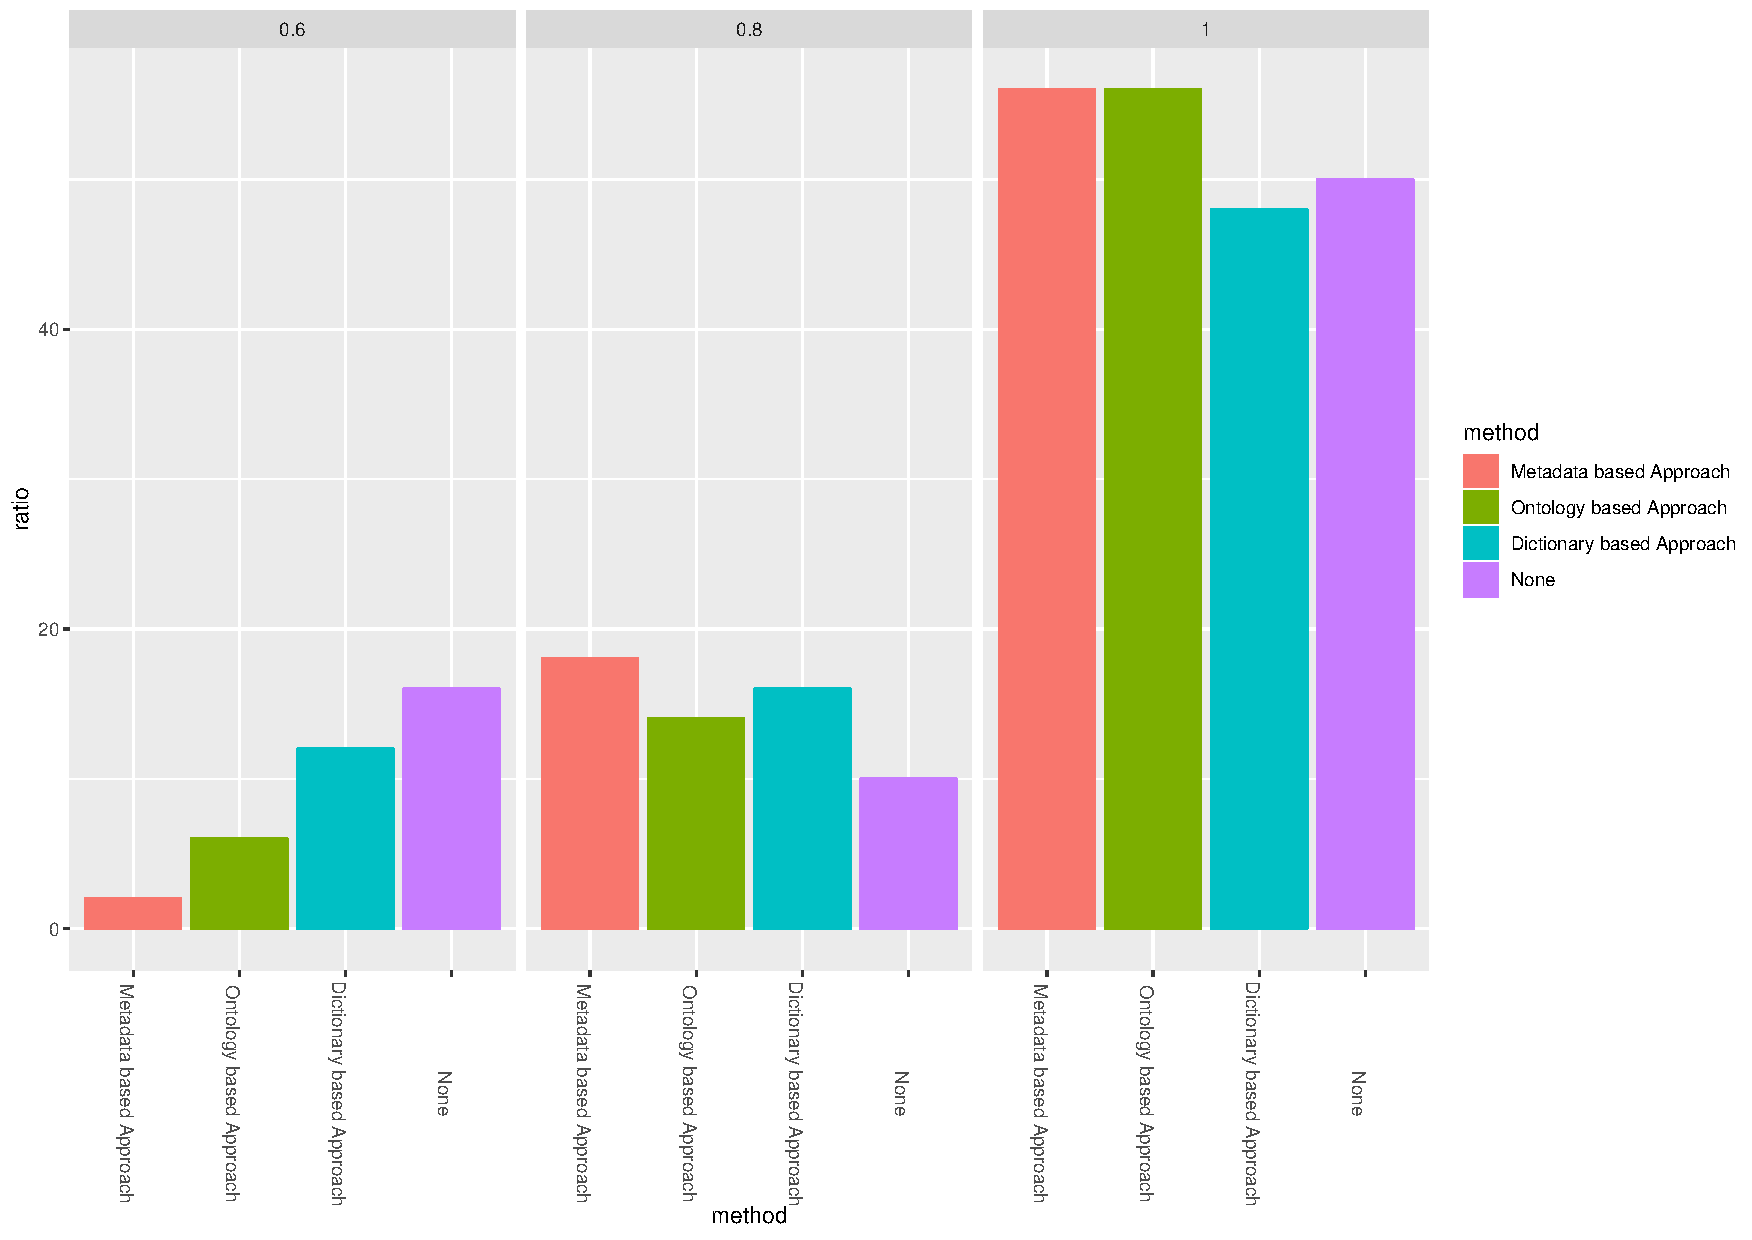
\includegraphics[width=\textwidth]{plots/finance/hist_agreement_corrected}
  	 \caption{Histogram plots of the Inter-rater Agreement}\label{fig:hist_agreement_finance_all}
\end{sidewaysfigure}
 
\begin{figure}
    \centering
    \begin{subfigure}[b]{0.4\textwidth}
        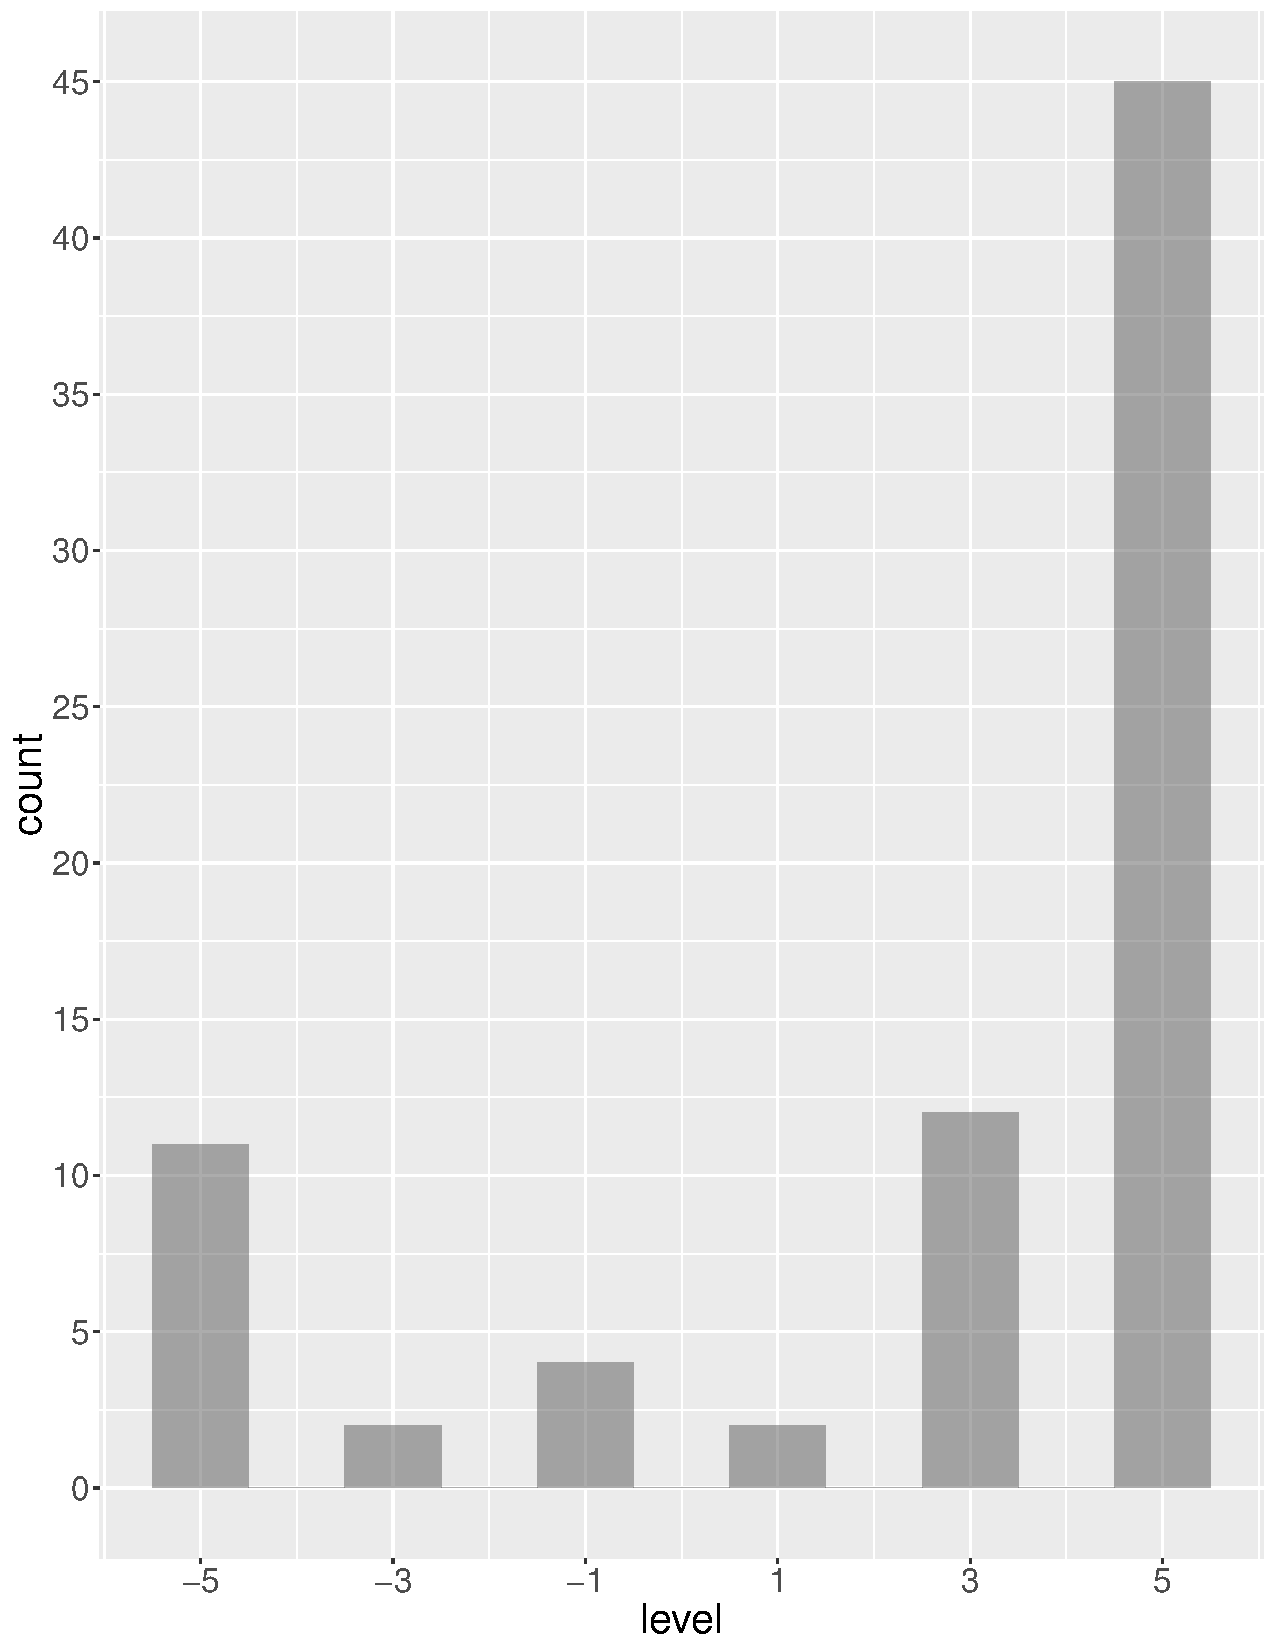
\includegraphics[width=\textwidth]{plots/finance/hist_level_nn}
        \caption{Ontology based Approach}
        \label{fig:hist_level_finance_nn}
    \end{subfigure}
    ~
    \begin{subfigure}[b]{0.4\textwidth}
        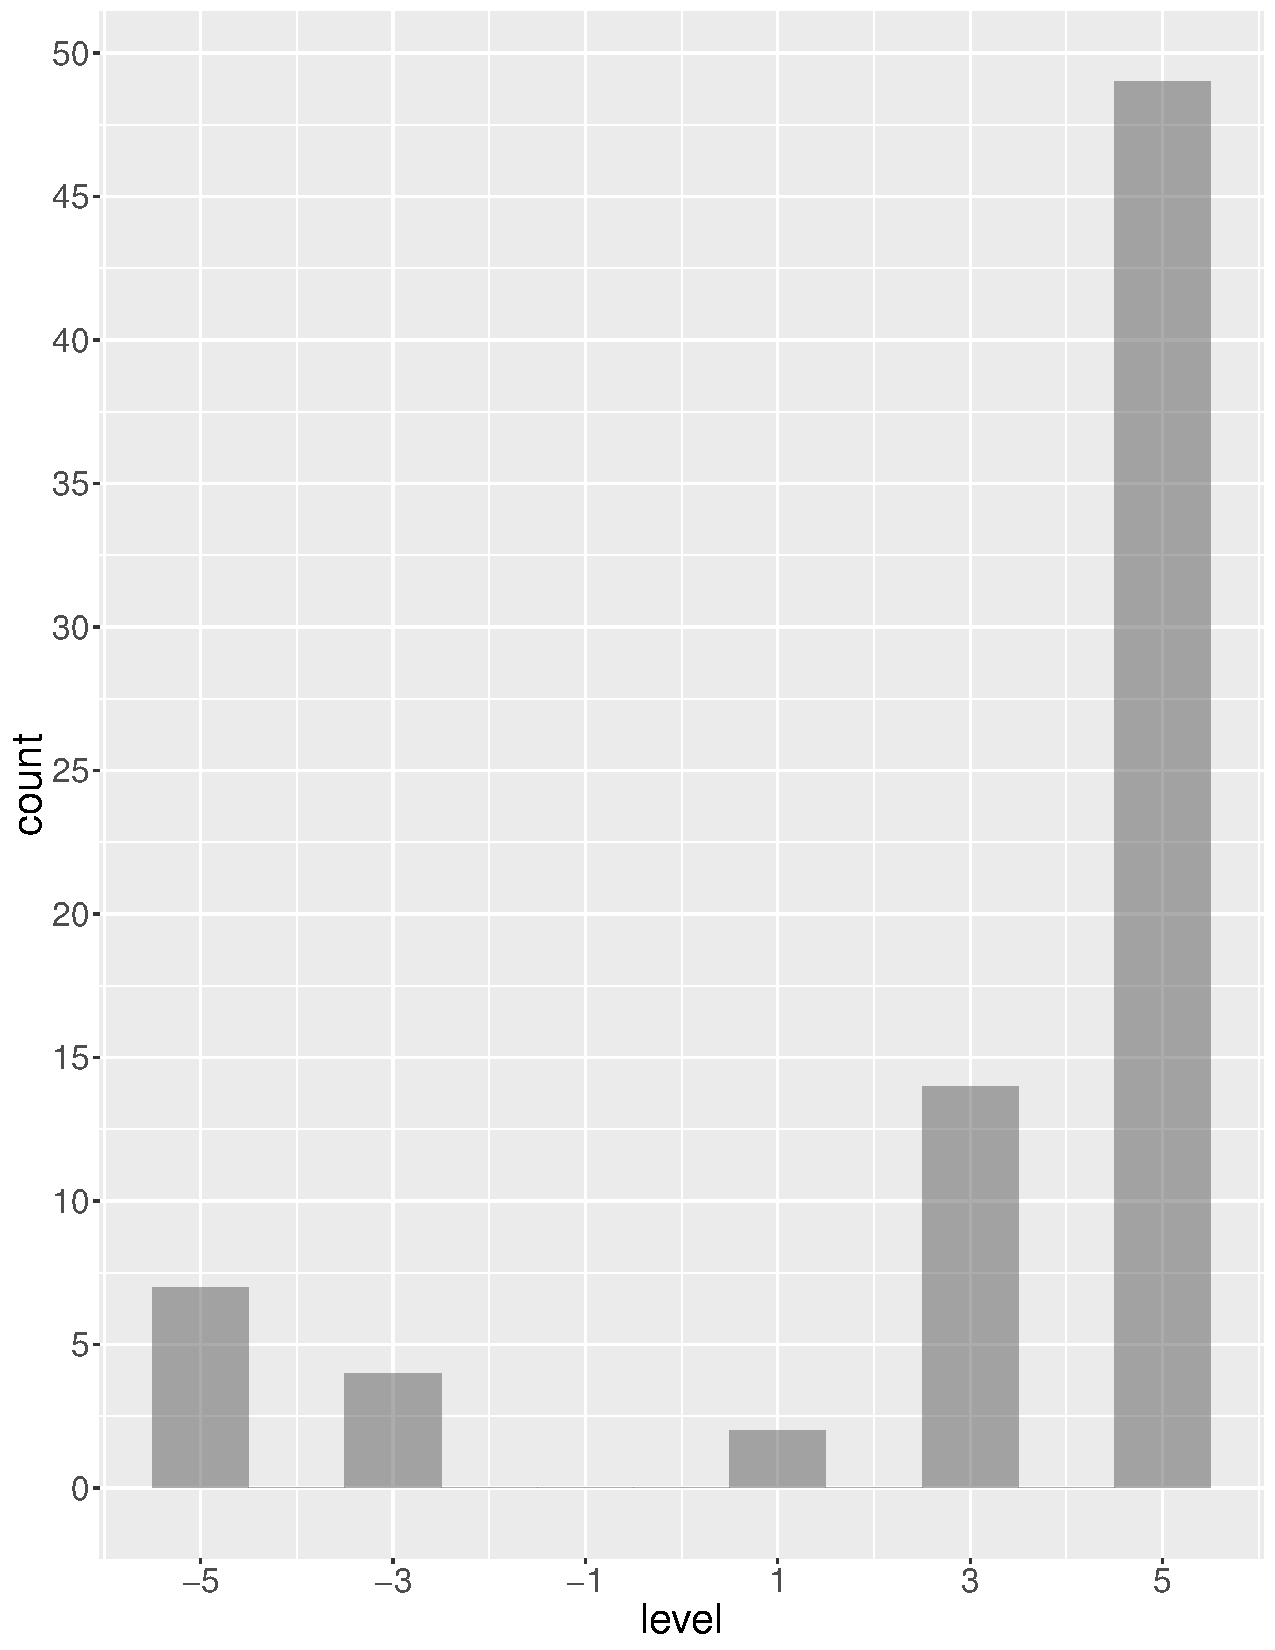
\includegraphics[width=\textwidth]{plots/finance/hist_level_ec}
        \caption{Metadata based Approach}
        \label{fig:hist_level_finance_ec}
    \end{subfigure}
    ~
    \begin{subfigure}[b]{0.4\textwidth}
        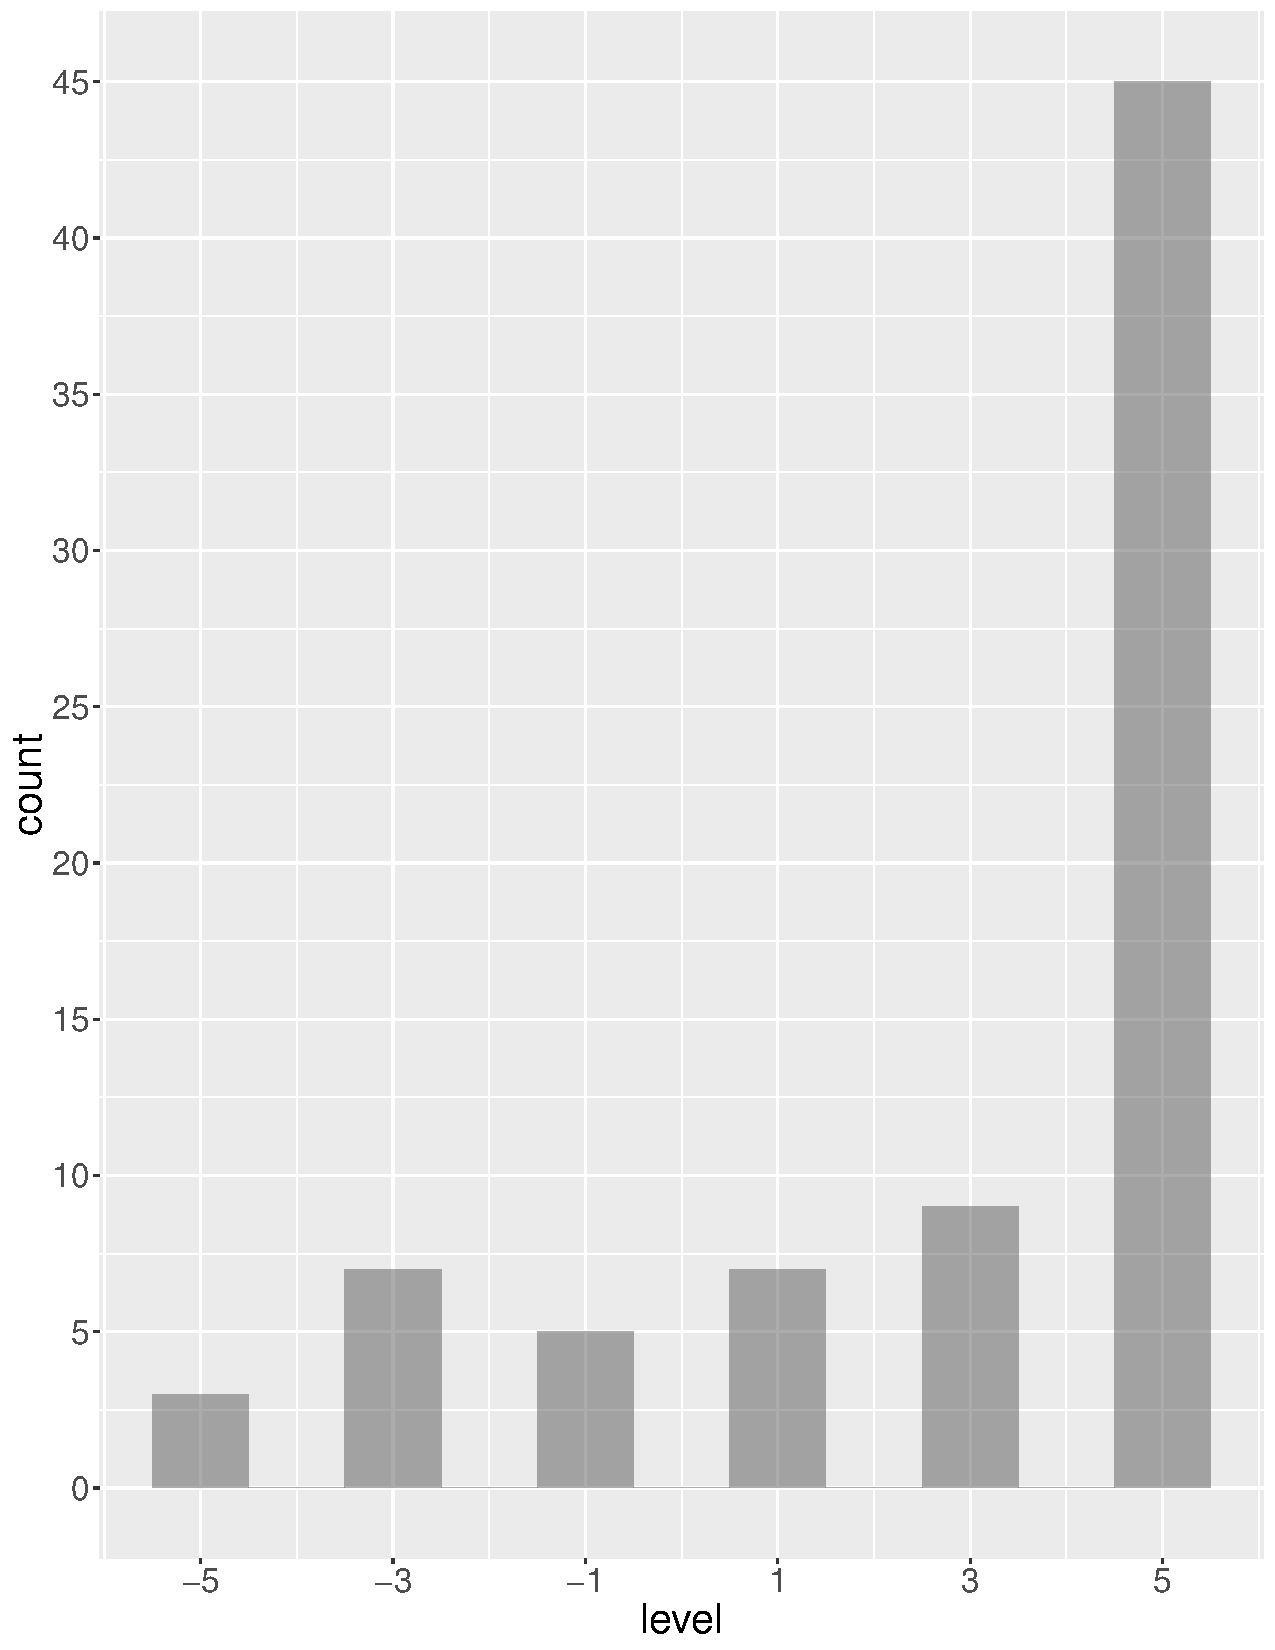
\includegraphics[width=\textwidth]{plots/finance/hist_level_es}
        \caption{Dictionary based Approach}
        \label{fig:hist_level_finance_es}
    \end{subfigure}
    ~
    \begin{subfigure}[b]{0.4\textwidth}
        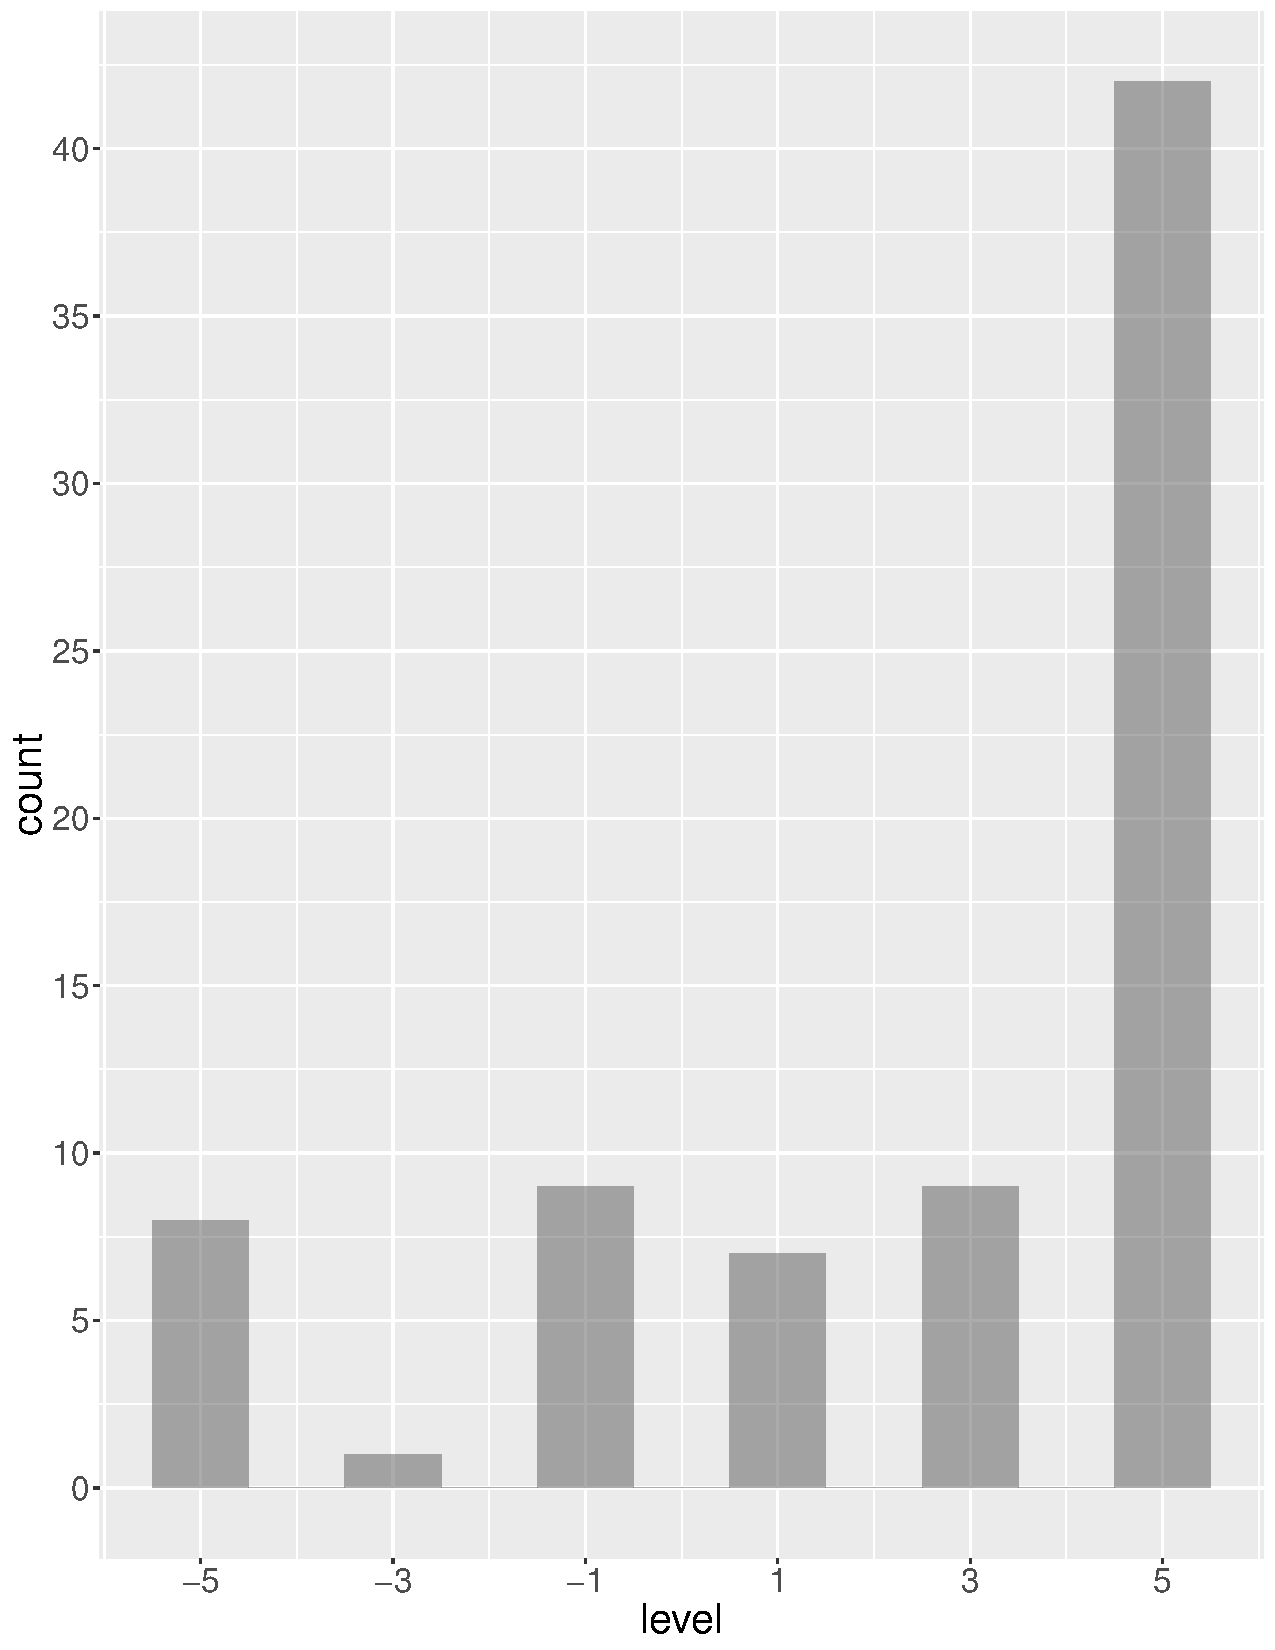
\includegraphics[width=\textwidth]{plots/finance/hist_level_none}
        \caption{None}
        \label{fig:hist_level_finance_none}
    \end{subfigure}
	\caption{Histogram plots of the correct/incorrect judgements. $\{$\emph{count}=number of judgements, \emph{level}=combined number of correct (positive scale) and incorrect (negative scale) judgements per concept$\}$ }
	\label{fig:hist_level_finance_all}
\end{figure}

To get a different view of the overall worker performance, \hyperref[fig:hist_level_finance_all]{Figure~\ref*{fig:hist_level_finance_all}} 
shows bar plots of the performance levels. Each level combines the agreement ratio with the amount of correct/incorrect judgements, yielding a higher score when most contributors agreed on correct answers and a lower score when they disagreed or answered incorrectly.
A common phenomena of all approaches was the high level of correct answers with high agreement across contributors. Indeed, this holds for the other datasets too. However, after analysing the concepts that were accepted and those that were declined, this is rather related to the generic nature of the used datasets. For example, whereas accepting the concept \emph{budget} for the finance domain is relatively easy even with no additional information, judging the concept \emph{world} is much more challenging. Therefore, judging generic concepts should be done better by domain experts who share a common understanding of the used vocabulary. 

\begingroup
\renewcommand{\arraystretch}{1.5}
\begin{table}
	\begin{tabularx}{\textwidth}{l c*{4}{Y}}
		\toprule
		Method & mean & median & $1^{st}$ quartile & $3^{rd}$ quartile \\
		\midrule
		 Metadata based Approach & 3.18 & 5.00 & 3.00 & 5.00 \\
		 Dictionary based Approach & 2.87 & 5.00 & 1.00 & 5.00 \\
		 Ontology based Approach & 2.61 & 5.00 & 2.50 & 5.00 \\
		 None & 2.53 & 5.00 & 1.00 & 5.00 \\
		\bottomrule
	\end{tabularx}
	\caption{Summary statistics concerning agreement level on the Finance Ontology~(ranked by mean value)}
	\label{table:level_corr_incorr_finance}
\end{table}
\endgroup

The summary statistics in~\hyperref[table:level_corr_incorr_finance]{Table~\ref*{table:level_corr_incorr_finance}} confirm our observations made so far. It shows the statistics of each method ranked by mean value. Judging the worker performance by the level of agreement and the ratio of correct/incorrect judgements, the order is no different than ranked by F-Measure. 


% SECTION: TENNIS ONTOLOGY %
\section{Tennis Ontology}\label{sec:result_t_ontology}
Reference to aggregated results~\hyperref[table:bench_p_r_f_tennis]{Table~\ref*{table:bench_p_r_f_tennis}}.
\begingroup
\renewcommand{\arraystretch}{1.5}
\begin{table}
	\begin{tabularx}{\textwidth}{l c*{3}{Y}}
		\toprule
		Method & Precision & Recall & F-Measure \\
		\midrule
		 Embedded Context & 0.896 & 0.976 & 0.934 \\
		 Neighbouring Nodes & 0.874 & 0.939 & 0.905 \\ 
		 None & 0.783 & 0.933 & 0.851 \\
		 External Source & 0.648 & 0.980 & 0.780 \\
		\bottomrule
	\end{tabularx}
	\caption{Aggregated results on the Tennis Ontology~(ranked by F-Measure)}
	\label{table:bench_p_r_f_tennis}
\end{table}
\endgroup

Reference to Inter-rater agreement plot~\hyperref[fig:hist_agreement_tennis_all]{Figure~\ref*{fig:hist_agreement_tennis_all}}.
\begin{sidewaysfigure}
  	 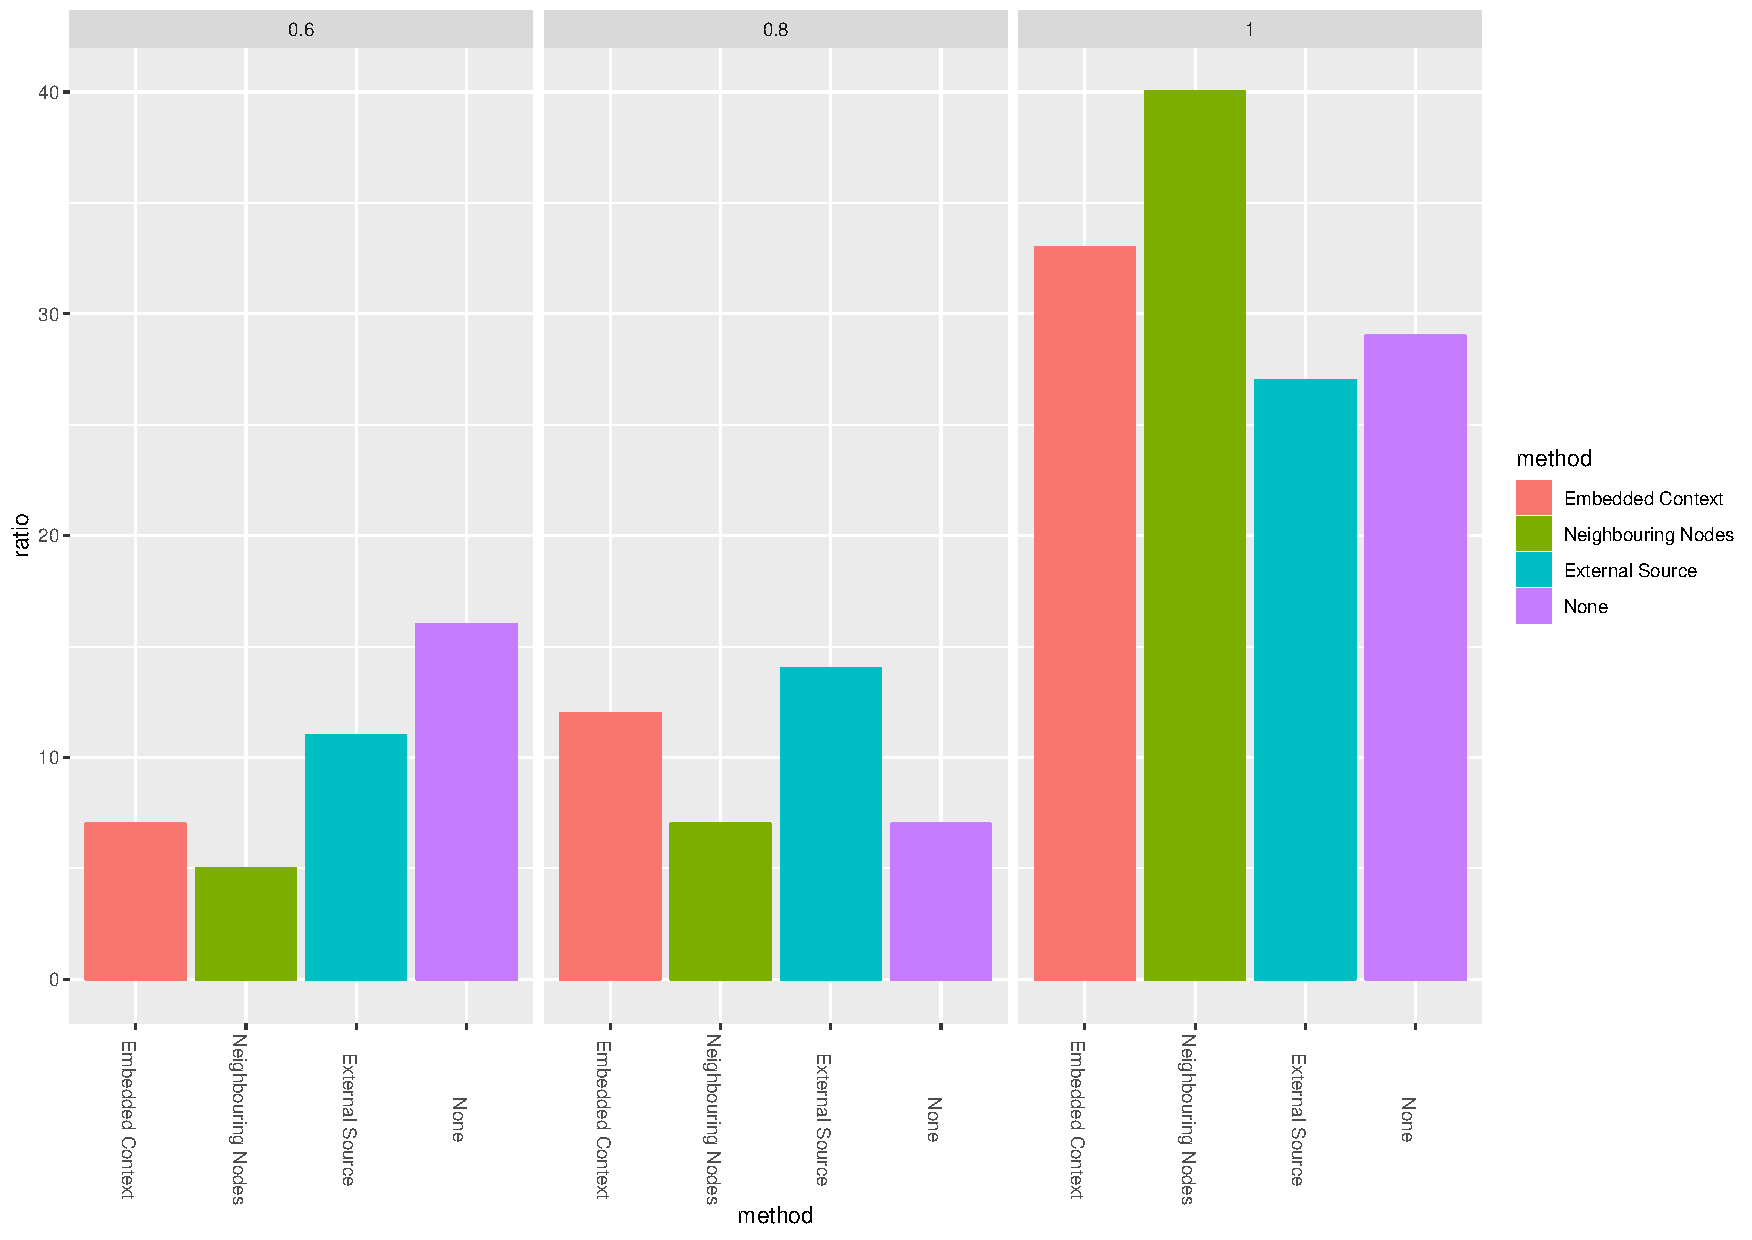
\includegraphics[width=\textwidth]{plots/tennis/hist_agreement}
  	 \caption{Histogram plots of the Inter-rater Agreement}\label{fig:hist_agreement_tennis_all}
\end{sidewaysfigure}



Reference to Histogram plots~\hyperref[fig:hist_level_tennis_all]{Figure~\ref*{fig:hist_level_tennis_all}}.
\begin{figure}
    \centering
    \begin{subfigure}[b]{0.4\textwidth}
        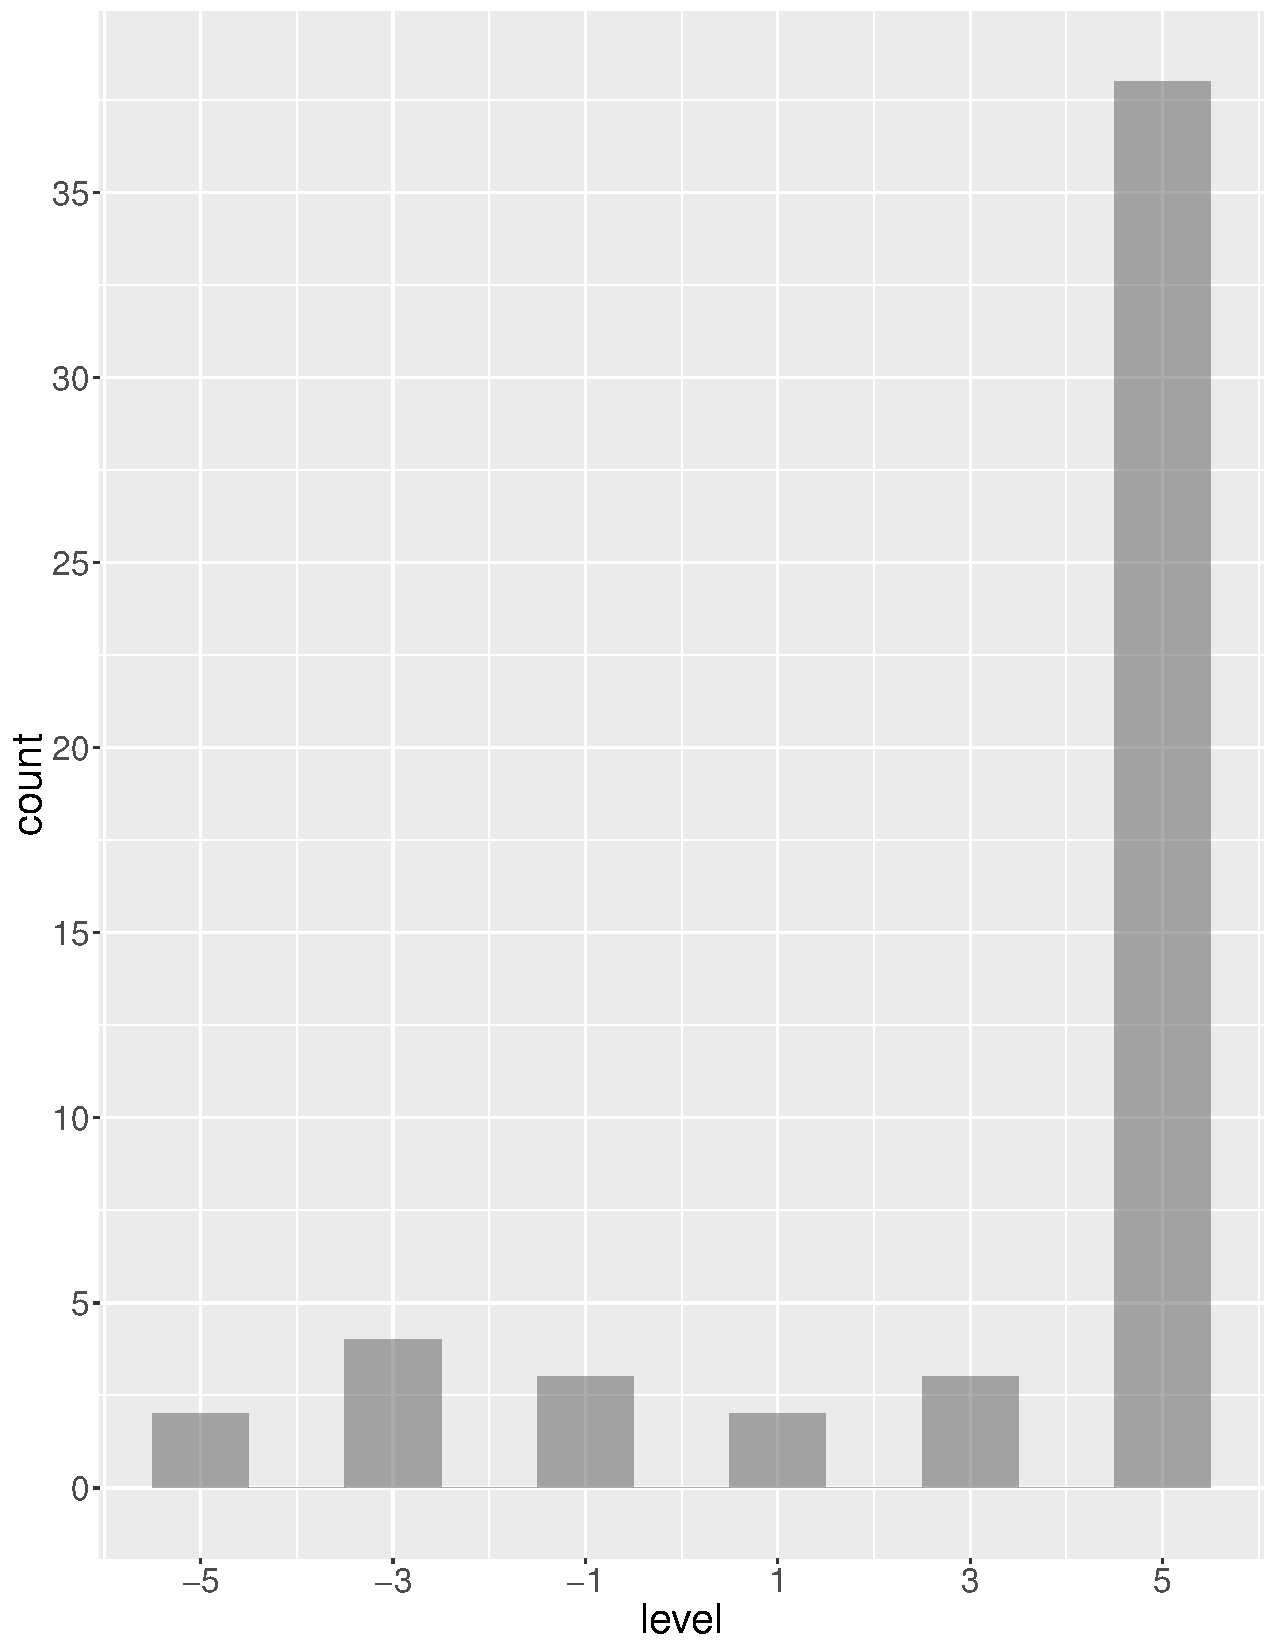
\includegraphics[width=\textwidth]{plots/tennis/hist_level_nn}
        \caption{Neighbouring Nodes}
        \label{fig:hist_level_tennis_nn}
    \end{subfigure}
    ~
    \begin{subfigure}[b]{0.4\textwidth}
        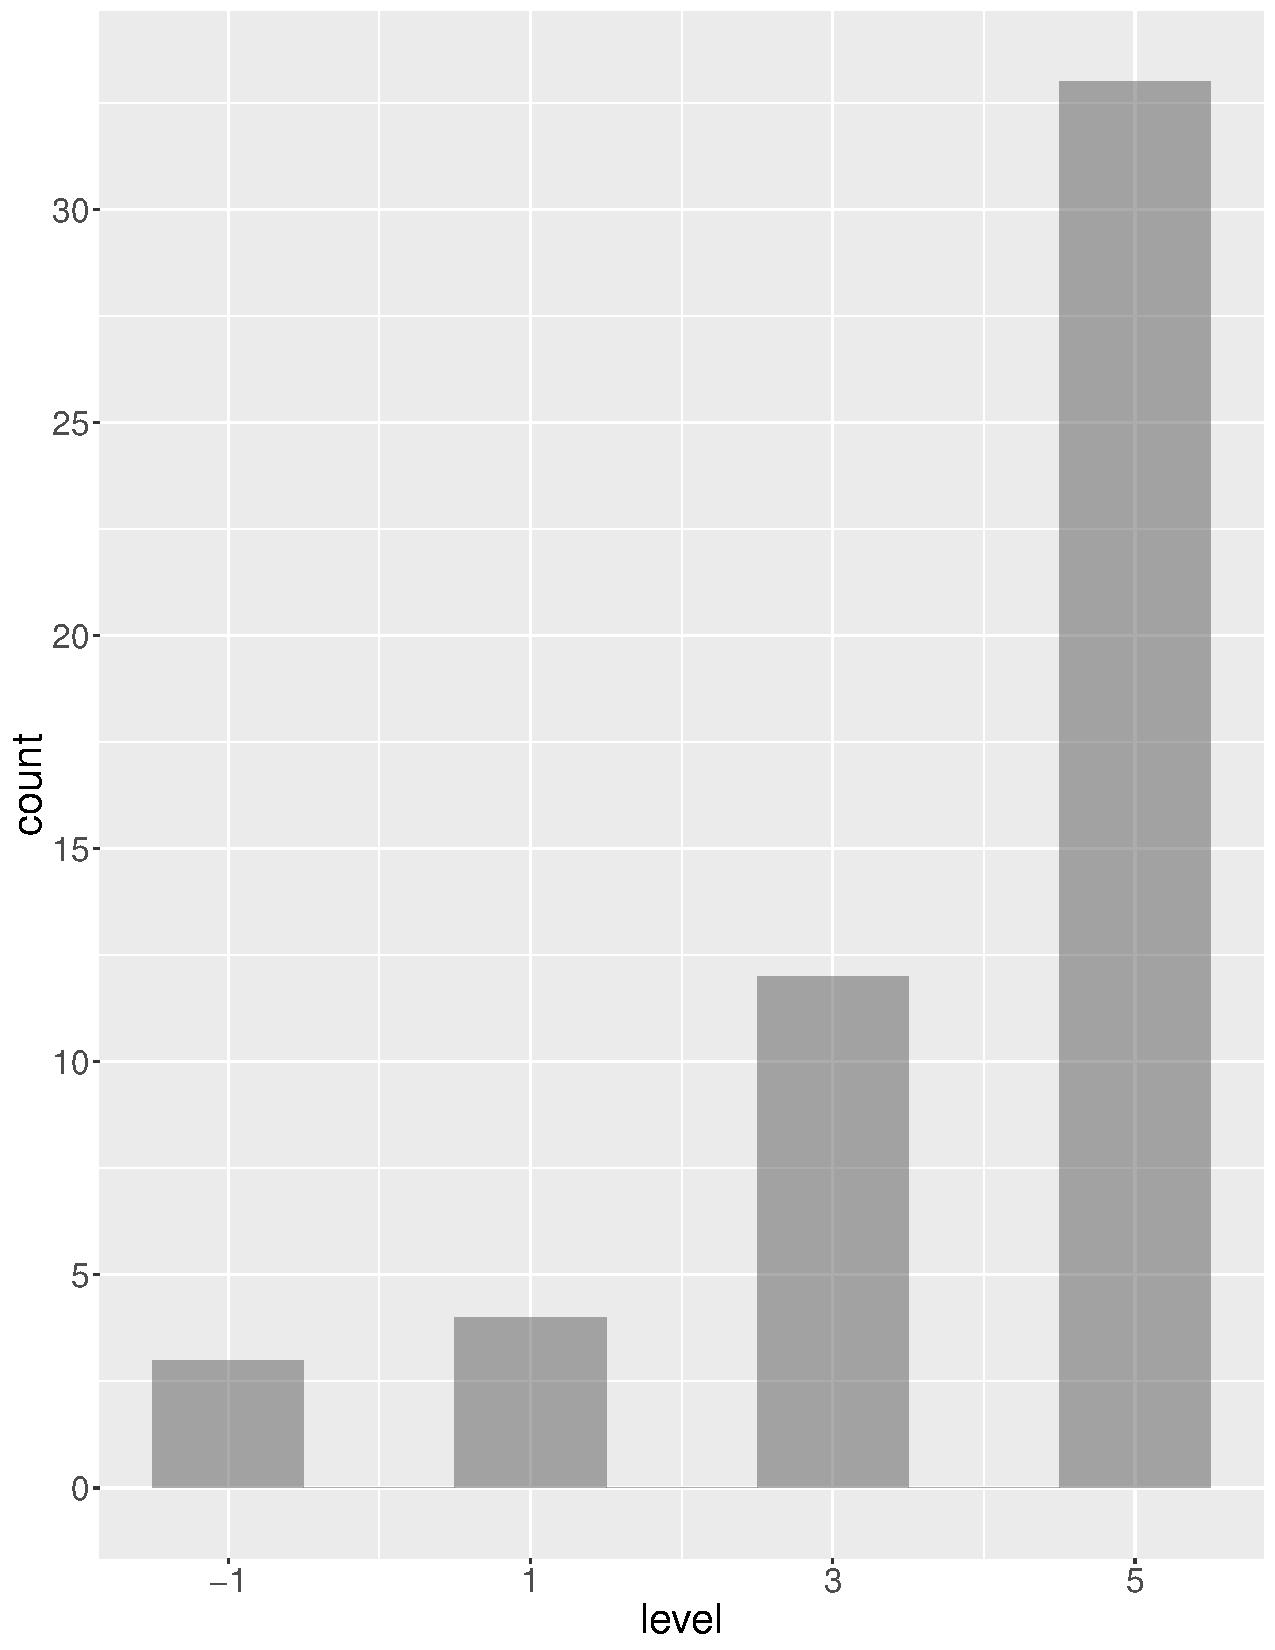
\includegraphics[width=\textwidth]{plots/tennis/hist_level_ec}
        \caption{Embedded Context}
        \label{fig:hist_level_tennis_ec}
    \end{subfigure}
    ~
    \begin{subfigure}[b]{0.4\textwidth}
        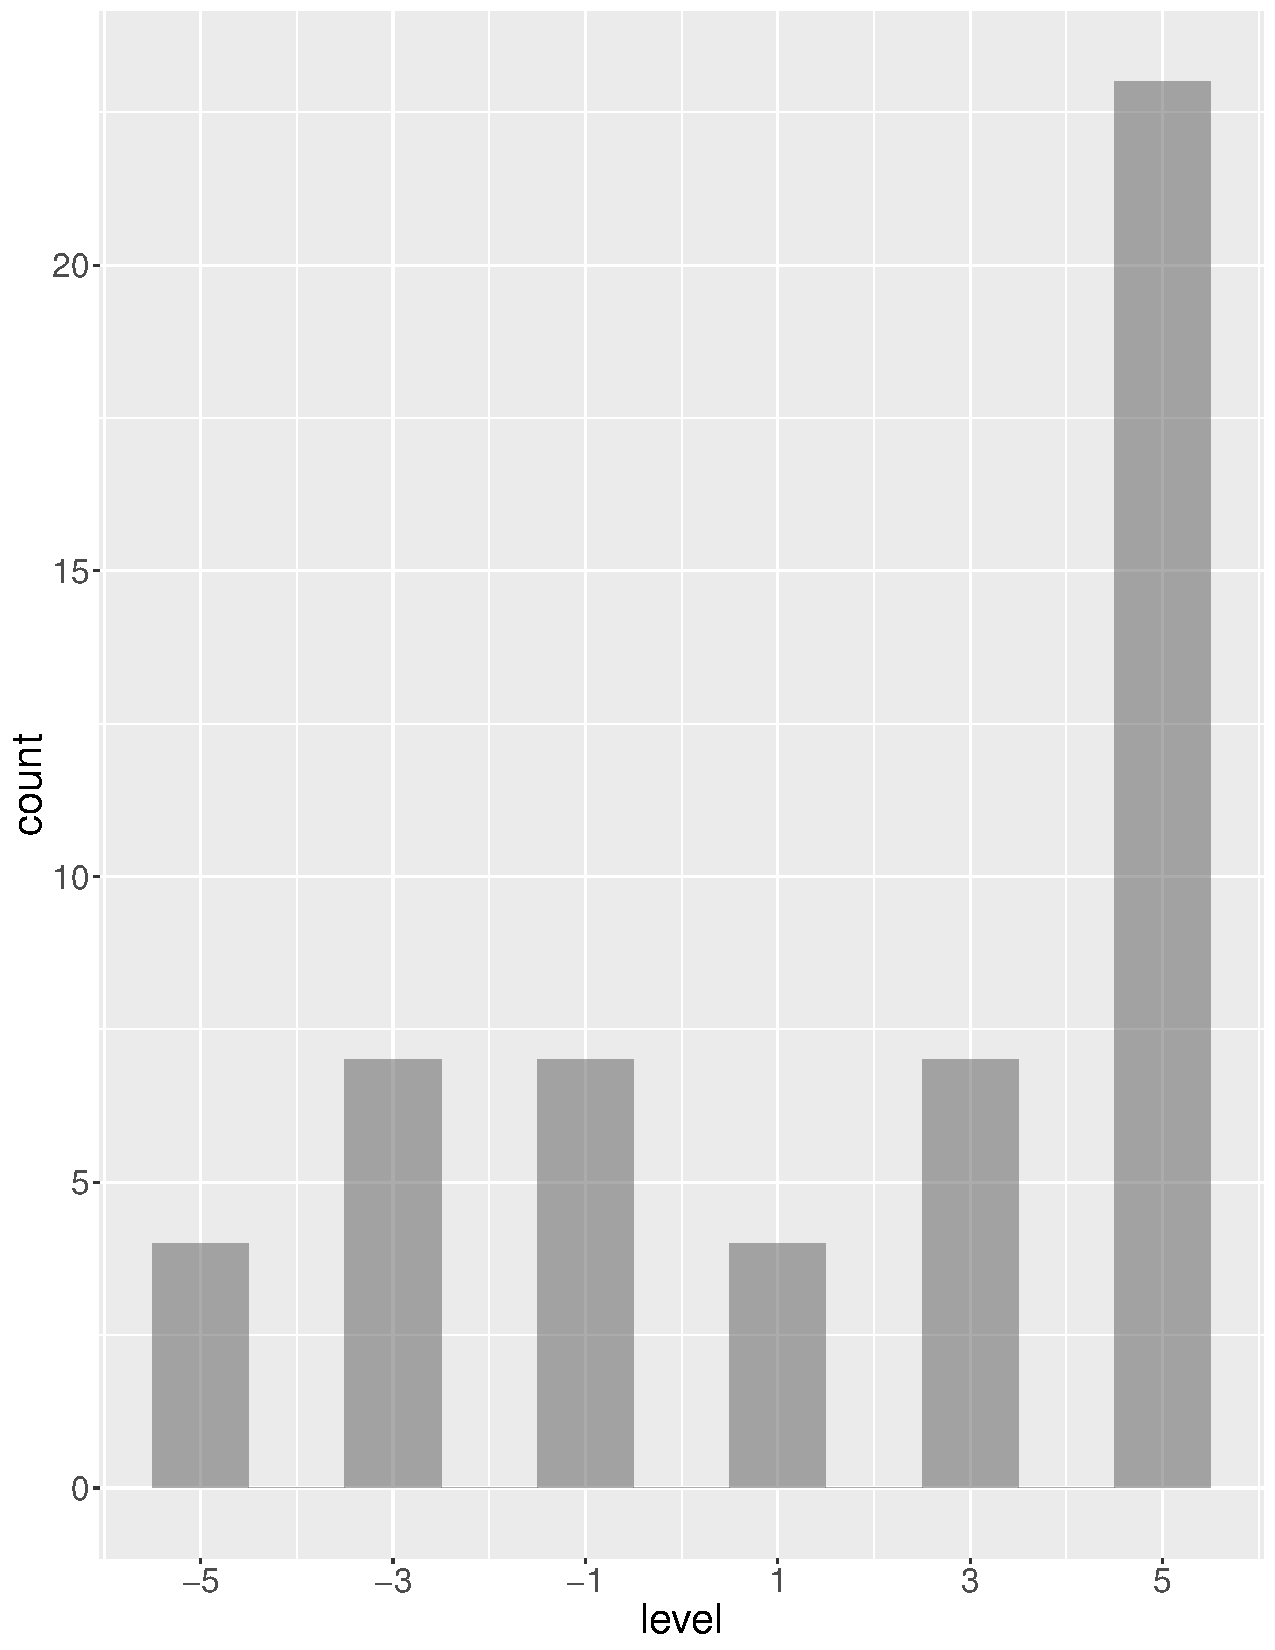
\includegraphics[width=\textwidth]{plots/tennis/hist_level_es}
        \caption{External Source}
        \label{fig:hist_level_tennis_es}
    \end{subfigure}
    ~
    \begin{subfigure}[b]{0.4\textwidth}
        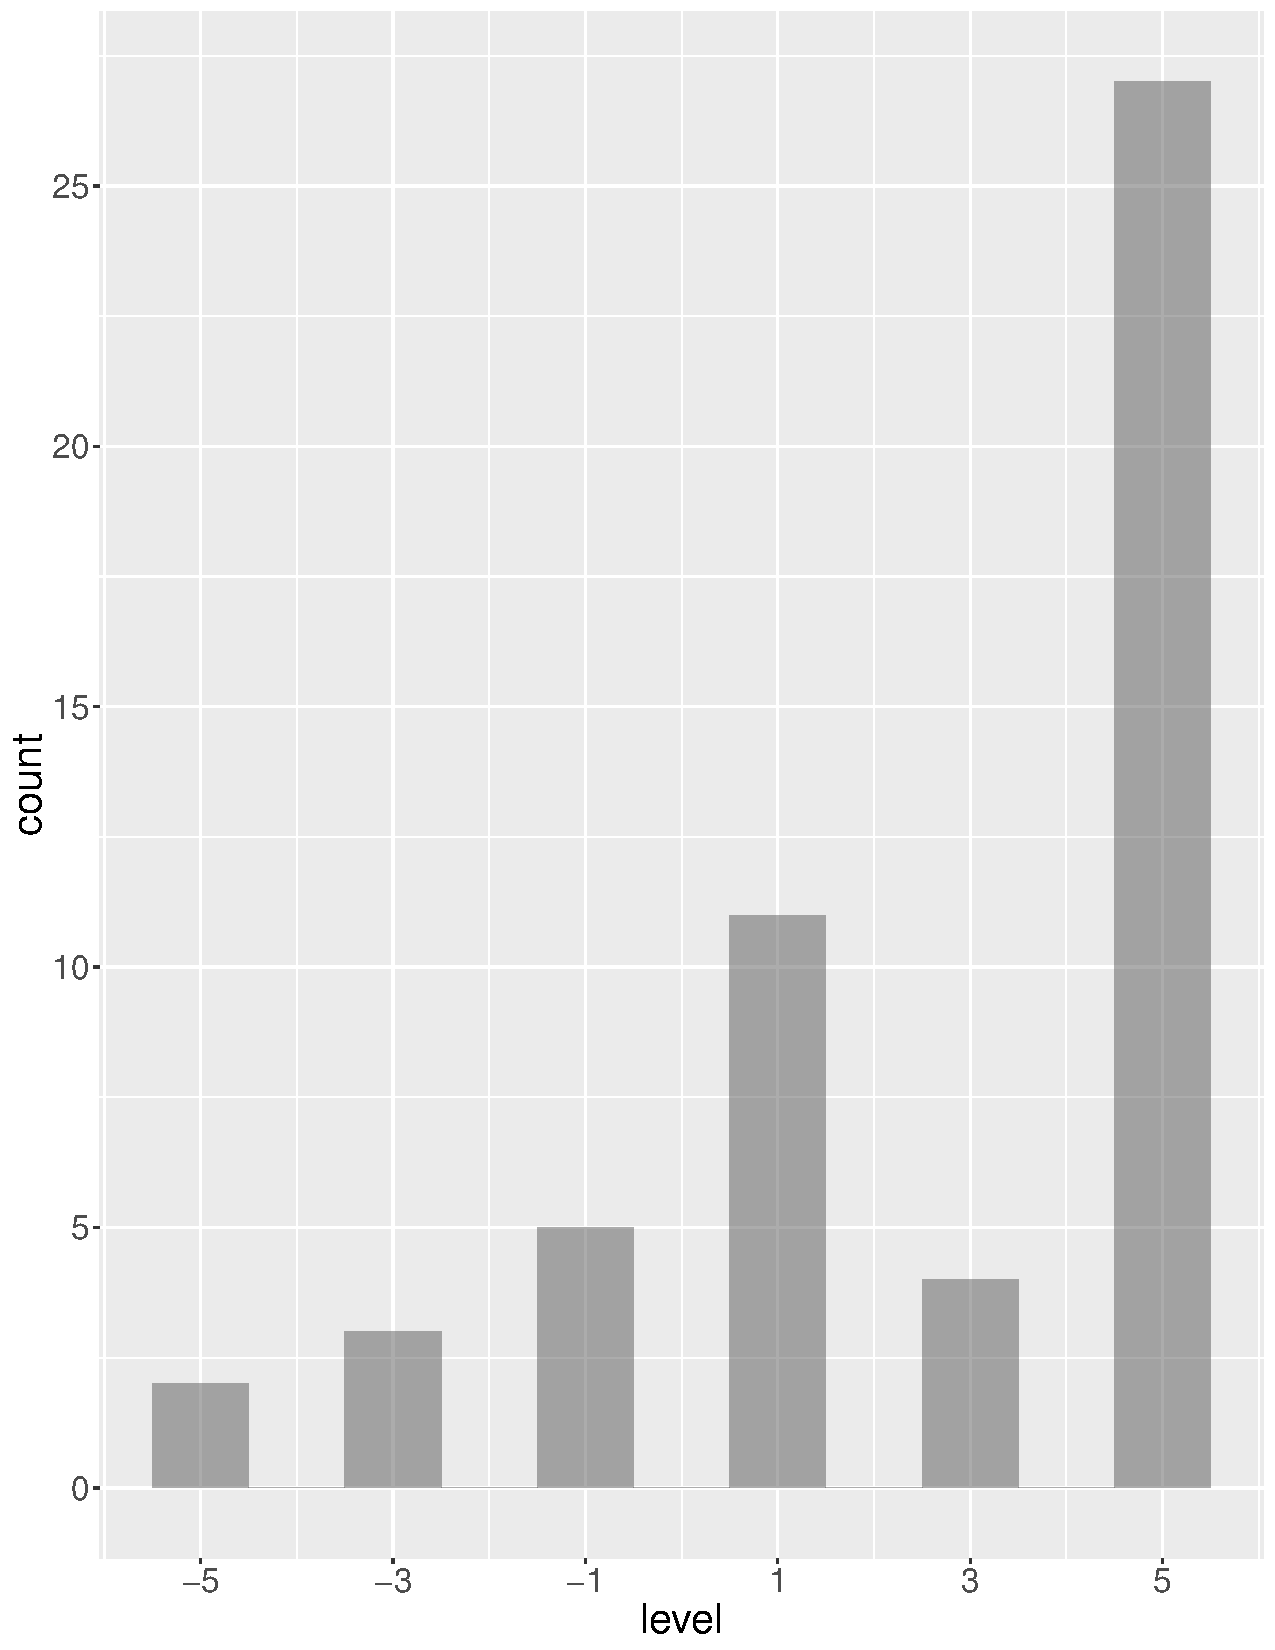
\includegraphics[width=\textwidth]{plots/tennis/hist_level_none}
        \caption{None}
        \label{fig:hist_level_tennis_none}
    \end{subfigure}
    \caption{Histogram plots of the correct/incorrect judgements}\label{fig:hist_level_tennis_all}
\end{figure}

Reference to agreement level~~\hyperref[table:level_corr_incorr_tennis]{Table~\ref*{table:level_corr_incorr_tennis}}.
\begingroup
\renewcommand{\arraystretch}{1.5}
\begin{table}
	\begin{tabularx}{\textwidth}{l c*{4}{Y}}
		\toprule
		Method & mean & median & $1^{st}$ quartile & $3^{rd}$ quartile \\
		\midrule
		 Embedded Context & 3.89 & 5.00 & 3.00 & 5.00 \\
		 Neighbouring Nodes & 3.39 & 5.00 & 3.00 & 5.00 \\
		 None & 2.58 & 5.00 & 1.00 & 5.00 \\
		 External Source & 1.77 & 3.00 & -1.00 & 5.00 \\
		\bottomrule
	\end{tabularx}
	\caption{Summary statistics concerning agreement level on the Finance Ontology~(ranked by mean value)}
	\label{table:level_corr_incorr_tennis}
\end{table}
\endgroup

% SECTION: EVALUATION COMPARISON %
\section{Evaluation Comparison}\label{sec:result_comparison}

\paragraph{Which Context Enrichment Method performed best in general?}
Lorem ipsum dolor sit amet, consectetur adipisicing elit, sed do eiusmod tempor incididunt ut labore et dolore magna aliqua. Ut enim ad minim veniam, quis nostrud exercitation ullamco laboris nisi ut aliquip ex ea commodo consequat. Duis aute irure dolor in reprehenderit in voluptate velit esse cillum dolore eu fugiat nulla pariatur. Excepteur sint occaecat cupidatat non proident, sunt in culpa qui officia deserunt mollit anim id est laborum.

\paragraph{Did the crowd perform better with context?}
Lorem ipsum dolor sit amet, consectetur adipisicing elit, sed do eiusmod tempor incididunt ut labore et dolore magna aliqua. Ut enim ad minim veniam, quis nostrud exercitation ullamco laboris nisi ut aliquip ex ea commodo consequat. Duis aute irure dolor in reprehenderit in voluptate velit esse cillum dolore eu fugiat nulla pariatur. Excepteur sint occaecat cupidatat non proident, sunt in culpa qui officia deserunt mollit anim id est laborum.

\paragraph{For which concepts were the crowd wrong?}
Lorem ipsum dolor sit amet, consectetur adipisicing elit, sed do eiusmod tempor incididunt ut labore et dolore magna aliqua. Ut enim ad minim veniam, quis nostrud exercitation ullamco laboris nisi ut aliquip ex ea commodo consequat. Duis aute irure dolor in reprehenderit in voluptate velit esse cillum dolore eu fugiat nulla pariatur. Excepteur sint occaecat cupidatat non proident, sunt in culpa qui officia deserunt mollit anim id est laborum.

\paragraph{Was there a correlation between Inter-rater Agreement and Accuracy}
Lorem ipsum dolor sit amet, consectetur adipisicing elit, sed do eiusmod tempor incididunt ut labore et dolore magna aliqua. Ut enim ad minim veniam, quis nostrud exercitation ullamco laboris nisi ut aliquip ex ea commodo consequat. Duis aute irure dolor in reprehenderit in voluptate velit esse cillum dolore eu fugiat nulla pariatur. Excepteur sint occaecat cupidatat non proident, sunt in culpa qui officia deserunt mollit anim id est laborum.

\paragraph{What other observations were found?}
Lorem ipsum dolor sit amet, consectetur adipisicing elit, sed do eiusmod tempor incididunt ut labore et dolore magna aliqua. Ut enim ad minim veniam, quis nostrud exercitation ullamco laboris nisi ut aliquip ex ea commodo consequat. Duis aute irure dolor in reprehenderit in voluptate velit esse cillum dolore eu fugiat nulla pariatur. Excepteur sint occaecat cupidatat non proident, sunt in culpa qui officia deserunt mollit anim id est laborum.

%%%%%%%%%%%%%%%%%%%%%%%%%%%%%%%%%%%%%%%%%%%%%%%%%%%%%%%%%%%%%%%%%%%%%%%%%%%%%%%%%%%%%%%%%%%%%%%%%%%%%%%%%%%%%%%%%%%%%%%%%%%%%%%%%%%%%%%%%%%%%%%%%%%%
